\documentclass[12pt]{article}
\usepackage{Sweave}
\usepackage{myVignette}
\usepackage[authoryear,round]{natbib}
\bibliographystyle{plainnat}
\DefineVerbatimEnvironment{Sinput}{Verbatim}
{formatcom={\vspace{-1.5ex}},fontshape=sl,
  fontfamily=courier,fontseries=b, fontsize=\scriptsize}
\DefineVerbatimEnvironment{Soutput}{Verbatim}
{formatcom={\vspace{-2.5ex}},fontfamily=courier,fontseries=b,%
  fontsize=\scriptsize}
%%\VignetteIndexEntry{Examples from Multilevel Software Reviews}
%%\VignetteDepends{lme4}
\begin{document}


\setkeys{Gin}{width=\textwidth}
\title{Examples from Multilevel Software Comparative Reviews}
\author{Douglas Bates\\R Development Core Team\\\email{Douglas.Bates@R-project.org}}
\date{\today}
\maketitle
\begin{abstract}
   The Center for Multilevel Modelling at the Institute of Education,
   London maintains a web site of ``Software reviews of multilevel
   modeling packages''.  The data sets discussed in the reviews are
   available at this web site.  We have incorporated these data sets
   in the \code{mlmRev} package for \RR{} and, in this vignette, provide
   the results of fitting several models to these data sets.
\end{abstract}

\section{Introduction}
\label{sec:Intro}

\RR{} is an Open Source implementation of John Chambers' \Slang{}
language for data analysis and graphics.  It was initially developed
by Ross Ihaka and Robert Gentleman of the University of Auckland and
now is developed and maintained by an international group of
statistical computing experts.

In addition to being Open Source software, which means that anyone can
examine the source code to see exactly how the computations are being
carried out, \RR{} is freely available from a network of archive sites
on the Internet.  There are precompiled versions for installation on
the Windows operating system, Mac OS X and several distributions of
the Linux operating system.  Because the source code is available
those interested in doing so can compile their own version if they wish.

\RR{} provides an environment for interactive computing with data and for
graphical display of data.  Users and developers can extend the
capabilities of \RR{} by writing their own functions in the language
and by creating packages of functions and data sets.  Many such
packages are available on the archive network called CRAN
(Comprehensive R Archive Network) for which the parent site is
\url{http://cran.r-project.org}. One such package called \code{lme4}
(along with a companion package called \code{Matrix}) provides
functions to fit and display linear mixed models and generalized
linear mixed models, which are the statisticians' names for the models
called multilevel models or hierarchical linear models in other
disciplines.  The \code{lattice} package provides functions to
generate several high level graphics plots that help with the
visualization of the types of data to which such models are fit.
Finally, the \code{mlmRev} package provides the data sets used in the
``Software Reviews of Multilevel Modeling Packages'' from the
Multilevel Modeling Group at the Institute of Education in the UK.
This package also contains several other data sets from the multilevel
modeling literature.

The software reviews mentioned above were intended to provide
comparison of the speed and accuracy of many different packages for
fitting multilevel models.  As such, there is a standard set of
models that fit to each of the data sets in each of the packages that
were capable of doing the fit.  We will fit these models for
comparative purposes but we will also do some graphical exploration of
the data and, in some cases, discuss alternative models.

We follow the general outline of the previous reviews, beginning with
simpler structures and moving to the more complex structures.  Because
the previous reviews were performed on older and considerably slower
computers than the ones on which this vignette will be compiled, the
timings produced by the \code{system.time} function and shown in the
text should not be compared with previous timings given on the web
site.  They are an indication of the times required to fit such models
to these data sets on recent computers with processors running at
around 2 GHz or faster.

\section{Two-level normal models}
\label{sec:TwoLevelNormal}

In the multilevel modeling literature a two-level model is one with
two levels of random variation; the per-observation noise term and
random effects which are grouped according to the levels of a factor.
We call this factor a \textit{grouping factor}. If the response is
measured on a continuous scale (more or less) our initial models are
based on a normal distribution for the per-observation noise and for
the random effects.  Thus such a model is called a ``two-level normal
model'' even though it has only one grouping factor for the random effects.


\subsection{The Exam data}
\label{sec:Examdata}

The data set called \code{Exam} provides the normalized exam scores
attained by 4,059 students from 65 schools in inner London.  Some of
the covariates available with this exam score are the school the
student attended, the sex of the student, the school gender (boys,
girls, or mixed) and the student's result on the Standardised London
Reading test.

The \RR{} functions \code{str} and \code{summary} can be used to
examine the structure of a data set (or, in general, any \RR{} object)
and to provide a summary of an object.
\begin{Schunk}
\begin{Sinput}
> str(Exam)
\end{Sinput}
\begin{Soutput}
`data.frame':	4059 obs. of  10 variables:
 $ school  : Factor w/ 65 levels "1","2","3","4",..: 1 1 1 1 1 1 1 1 1 1 ...
 $ normexam: num   0.261  0.134 -1.724  0.968  0.544 ...
 $ schgend : Factor w/ 3 levels "mixed","boys",..: 1 1 1 1 1 1 1 1 1 1 ...
 $ schavg  : num  0.166 0.166 0.166 0.166 0.166 ...
 $ vr      : Factor w/ 3 levels "bottom 25%","mid 50%",..: 2 2 2 2 2 2 2 2 2 2 ...
 $ intake  : Factor w/ 3 levels "bottom 25%","mid 50%",..: 1 2 3 2 2 1 3 2 2 3 ...
 $ standLRT: num   0.619  0.206 -1.365  0.206  0.371 ...
 $ sex     : Factor w/ 2 levels "F","M": 1 1 2 1 1 2 2 2 1 2 ...
 $ type    : Factor w/ 2 levels "Mxd","Sngl": 1 1 1 1 1 1 1 1 1 1 ...
 $ student : Factor w/ 650 levels "1","2","3","4",..: 143 145 142 141 138 155 158 115 117 113 ...
\end{Soutput}
\begin{Sinput}
> summary(Exam)
\end{Sinput}
\begin{Soutput}
     school        normexam           schgend         schavg         
 14     : 198   Min.   :-3.6660720   mixed:2169   Min.   :-0.755961  
 17     : 126   1st Qu.:-0.6995050   boys : 513   1st Qu.:-0.149341  
 18     : 120   Median : 0.0043222   girls:1377   Median :-0.020198  
 49     : 113   Mean   :-0.0001138                Mean   : 0.001810  
 8      : 102   3rd Qu.: 0.6787592                3rd Qu.: 0.210525  
 15     :  91   Max.   : 3.6660912                Max.   : 0.637656  
 (Other):3309                                                        
          vr              intake        standLRT         sex        type     
 bottom 25%: 640   bottom 25%:1176   Min.   :-2.934953   F:2436   Mxd :2169  
 mid 50%   :2263   mid 50%   :2344   1st Qu.:-0.620713   M:1623   Sngl:1890  
 top 25%   :1156   top 25%   : 539   Median : 0.040499                       
                                     Mean   : 0.001810                       
                                     3rd Qu.: 0.619059                       
                                     Max.   : 3.015952                       
                                                                             
    student    
 20     :  34  
 54     :  34  
 15     :  33  
 22     :  33  
 31     :  33  
 59     :  33  
 (Other):3859  
\end{Soutput}
\end{Schunk}


\subsection{Model fits and timings}
\label{sec:ExamFits}

The first model to fit to the Exam data incorporates fixed-effects
terms for the pretest score, the student's sex and the school gender.
The only random-effects term is an additive shift associated with the
school.

\begin{Schunk}
\begin{Sinput}
> (Em1 <- lmer(normexam ~ standLRT + sex + schgend + (1 | school), 
+     Exam))
\end{Sinput}
\begin{Soutput}
Linear mixed-effects model fit by REML
Formula: normexam ~ standLRT + sex + schgend + (1 | school) 
   Data: Exam 
      AIC      BIC    logLik MLdeviance REMLdeviance
 9361.673 9405.834 -4673.837   9325.501     9347.673
Random effects:
 Groups   Name        Variance Std.Dev.
 school   (Intercept) 0.085829 0.29297 
 Residual             0.562534 0.75002 
# of obs: 4059, groups: school, 65

Fixed effects:
                Estimate  Std. Error   DF t value  Pr(>|t|)
(Intercept)  -1.0493e-03  5.5569e-02 4054 -0.0189   0.98494
standLRT      5.5975e-01  1.2450e-02 4054 44.9601 < 2.2e-16
sexM         -1.6739e-01  3.4100e-02 4054 -4.9089 9.519e-07
schgendboys   1.7769e-01  1.1347e-01 4054  1.5659   0.11745
schgendgirls  1.5900e-01  8.9403e-02 4054  1.7784   0.07541
\end{Soutput}
\end{Schunk}

The \code{system.time} function can be used to time the execution of
an \RR{} expression.  It returns a vector of five numbers giving the
user time (time spend executing applications code), the system time
(time spent executing system functions called by the applications
code), the elapsed time, and the user and system time for any child
processes.  The first number is what is commonly viewed as the time
required to do the model fit.  (The elapsed time is unsuitable because
it can be affected by other processes running on the computer.)  These
times are in seconds.  On modern computers this fit takes only a
fraction of a second.

\begin{Schunk}
\begin{Sinput}
> system.time(lmer(normexam ~ standLRT + sex + schgend + (1 | school), 
+     Exam))
\end{Sinput}
\begin{Soutput}
[1] 0.09 0.00 0.08 0.00 0.00
\end{Soutput}
\end{Schunk}



\subsection{Interpreting the fit}
\label{sec:ExamInterpret}

As can be seen from the output, the default method of fitting a linear
mixed model is restricted maximum likelihood (REML).  The estimates of
the variance components correspond to those reported by other packages
as given on the Multilevel Modelling Group's web site.  Note that the
estimates of the variance components are given on the scale of the
variance and on the scale of the standard deviation.  That is, the
values in the column headed \code{Std.Dev.} are simply the square
roots of the corresponding entry in the \code{Variance} column.  They
are \textbf{not} standard errors of the estimate of the variance.

The estimates of the fixed-effects are different from those quoted on
the web site because the terms for \code{sex} and \code{schgend} use a
different parameterization than in the reviews.  Here the reference
level of \code{sex} is female (\code{F}) and the coefficient labelled
\code{sexM} represents the difference for males compared to females.
Similarly the reference level of \code{schgend} is \code{mixed} and
the two coefficients represent the change from mixed to boys only and
the change from mixed to girls only.  The value of the coefficient
labelled \code{Intercept} is affected by both these changes as is the
value of the REML criterion.

To reproduce the results obtained from other packages, we must change
the reference level for each of these factors.

\begin{Schunk}
\begin{Sinput}
> Exam$sex <- relevel(Exam$sex, "M")
> Exam$schgend <- relevel(Exam$schgend, "girls")
> (Em2 <- lmer(normexam ~ standLRT + sex + schgend + (1 | school), 
+     Exam))
\end{Sinput}
\begin{Soutput}
Linear mixed-effects model fit by REML
Formula: normexam ~ standLRT + sex + schgend + (1 | school) 
   Data: Exam 
      AIC      BIC    logLik MLdeviance REMLdeviance
 9361.673 9405.834 -4673.837   9325.501     9347.673
Random effects:
 Groups   Name        Variance Std.Dev.
 school   (Intercept) 0.085829 0.29297 
 Residual             0.562534 0.75002 
# of obs: 4059, groups: school, 65

Fixed effects:
                Estimate  Std. Error   DF t value  Pr(>|t|)
(Intercept)    -0.009444    0.077896 4054 -0.1212   0.90351
standLRT        0.559755    0.012450 4054 44.9601 < 2.2e-16
sexF            0.167391    0.034100 4054  4.9089 9.519e-07
schgendmixed   -0.158997    0.089403 4054 -1.7784   0.07541
schgendboys     0.018694    0.126058 4054  0.1483   0.88212
\end{Soutput}
\end{Schunk}

The coefficients now correspond to those in the tables on the web
site.  It happens that the REML criterion at the optimum in this fit
is the same as in the previous fit, but you cannot depend on this
occuring.  In general the value of the REML criterion at the optimum
depends on the parameterization used for the fixed effects.

\subsection{Further exploration}
\label{sec:ExamExplore}


\subsubsection{Checking consistency of the data}
\label{sec:consistency}

It is important to check the consistency of data before trying to fit
sophisticated models.  One should plot the data in many different ways
to see if it looks reasonableand also check relationships between
variables.  

For example, each observation in these data is associated with a
particular student.  The variable \code{student} is not a unique
identifier of the student as it only has 650 unique values.  It is
intended to be a unique identifier within a school but it is not.  To
show this we create a factor that is the interaction of school and
student then drop unused levels.

\begin{Schunk}
\begin{Sinput}
> Exam$ids <- with(Exam, school:student)[, drop = TRUE]
> str(Exam)
\end{Sinput}
\begin{Soutput}
`data.frame':	4059 obs. of  11 variables:
 $ school  : Factor w/ 65 levels "1","2","3","4",..: 1 1 1 1 1 1 1 1 1 1 ...
 $ normexam: num   0.261  0.134 -1.724  0.968  0.544 ...
 $ schgend : Factor w/ 3 levels "girls","mixed",..: 2 2 2 2 2 2 2 2 2 2 ...
 $ schavg  : num  0.166 0.166 0.166 0.166 0.166 ...
 $ vr      : Factor w/ 3 levels "bottom 25%","mid 50%",..: 2 2 2 2 2 2 2 2 2 2 ...
 $ intake  : Factor w/ 3 levels "bottom 25%","mid 50%",..: 1 2 3 2 2 1 3 2 2 3 ...
 $ standLRT: num   0.619  0.206 -1.365  0.206  0.371 ...
 $ sex     : Factor w/ 2 levels "M","F": 2 2 1 2 2 1 1 1 2 1 ...
 $ type    : Factor w/ 2 levels "Mxd","Sngl": 1 1 1 1 1 1 1 1 1 1 ...
 $ student : Factor w/ 650 levels "1","2","3","4",..: 143 145 142 141 138 155 158 115 117 113 ...
 $ ids     : Factor w/ 4055 levels "1:1","1:4","1:6",..: 48 49 47 46 45 50 51 39 40 38 ...
\end{Soutput}
\end{Schunk}

Notice that there are 4059 observations but only 4055 unique levels of
student within school.  We can check the ones that are duplicated

\begin{Schunk}
\begin{Sinput}
> as.character(Exam$ids[which(duplicated(Exam$ids))])
\end{Sinput}
\begin{Soutput}
[1] "43:86" "50:39" "52:2"  "52:21"
\end{Soutput}
\end{Schunk}

One of these cases
\begin{Schunk}
\begin{Sinput}
> subset(Exam, ids == "43:86")
\end{Sinput}
\begin{Soutput}
     school   normexam schgend    schavg      vr  intake   standLRT sex type
2758     43 -0.8526700   mixed 0.4334322 top 25% mid 50%  0.1231502   M  Mxd
2759     43  0.8219882   mixed 0.4334322 top 25% top 25% -0.0421520   F  Mxd
     student   ids
2758      86 43:86
2759      86 43:86
\end{Soutput}
\begin{Sinput}
> xtabs(~sex + school, Exam, subset = school %in% c(43, 50, 52), 
+     drop = TRUE)
\end{Sinput}
\begin{Soutput}
   school
sex 43 50 52
  M  1 35 61
  F 60 38  0
\end{Soutput}
\end{Schunk}
is particularly interesting.  Notice that one of the students
numbered 86 in school 43 is the only male student out of 61 students
from this school who took the exam.  It is quite likely that this
student's score was attributed to the wrong school and that the school
is in fact a girls-only school, not a mixed-sex school.

The causes of the other three cases of duplicate student numbers
within a school are not as clear.  It would be necessary to go back
to the original data records to check these.

The cross-tabulation of the students by sex and school for the
mixed-sex schools
\begin{Schunk}
\begin{Sinput}
> xtabs(~sex + school, Exam, subset = type == "Mxd", drop = TRUE)
\end{Sinput}
\begin{Soutput}
   school
sex   1   3   4   5   9  10  12  13  14  15  17  19  20  22  23  26  28  32  33
  M  45  29  45  16  21  31  23  26  92  47  31  33  21  48  10  44  31  27  44
  F  28  23  34  19  13  19  24  38 106  44  95  22  18  42  18  31  26  15  33
   school
sex  34  38  42  43  45  46  47  50  51  54  55  56  59  61  62  63
  M  18  31  35   1   5  47  81  35  26   4  26  16  30  35  43  13
  F   8  23  23  60  48  36   1  38  32   4  25  22  17  29  28  17
\end{Soutput}
\end{Schunk}
shows another anomaly.  School 47 is similar to school 43 in that,
although it is classified as a mixed-sex school, 81 male students
and only one female student took the exam.  It is likely that the
school was misrecorded for this one female student and the school is a
male-only school.  

Another school is worth noting. There were only eight students from
school 54 who took the exam so any within-school estimates from this
school will be unreliable.

A mosaic plot (Figure~\ref{fig:ExamMosaic}) produced with
\begin{Schunk}
\begin{Sinput}
> library(vcd)
> ExamMxd <- subset(Exam, type == "Mxd")
> ExamMxd$school <- ExamMxd$school[, drop = TRUE]
> mosaic(~school + sex, ExamMxd, shade = TRUE)
\end{Sinput}
\end{Schunk}
helps to detect mixed-sex schools with unusually large or unusually small ratios
of females to males taking the exam.
\begin{figure}[tbp]
  \centering
  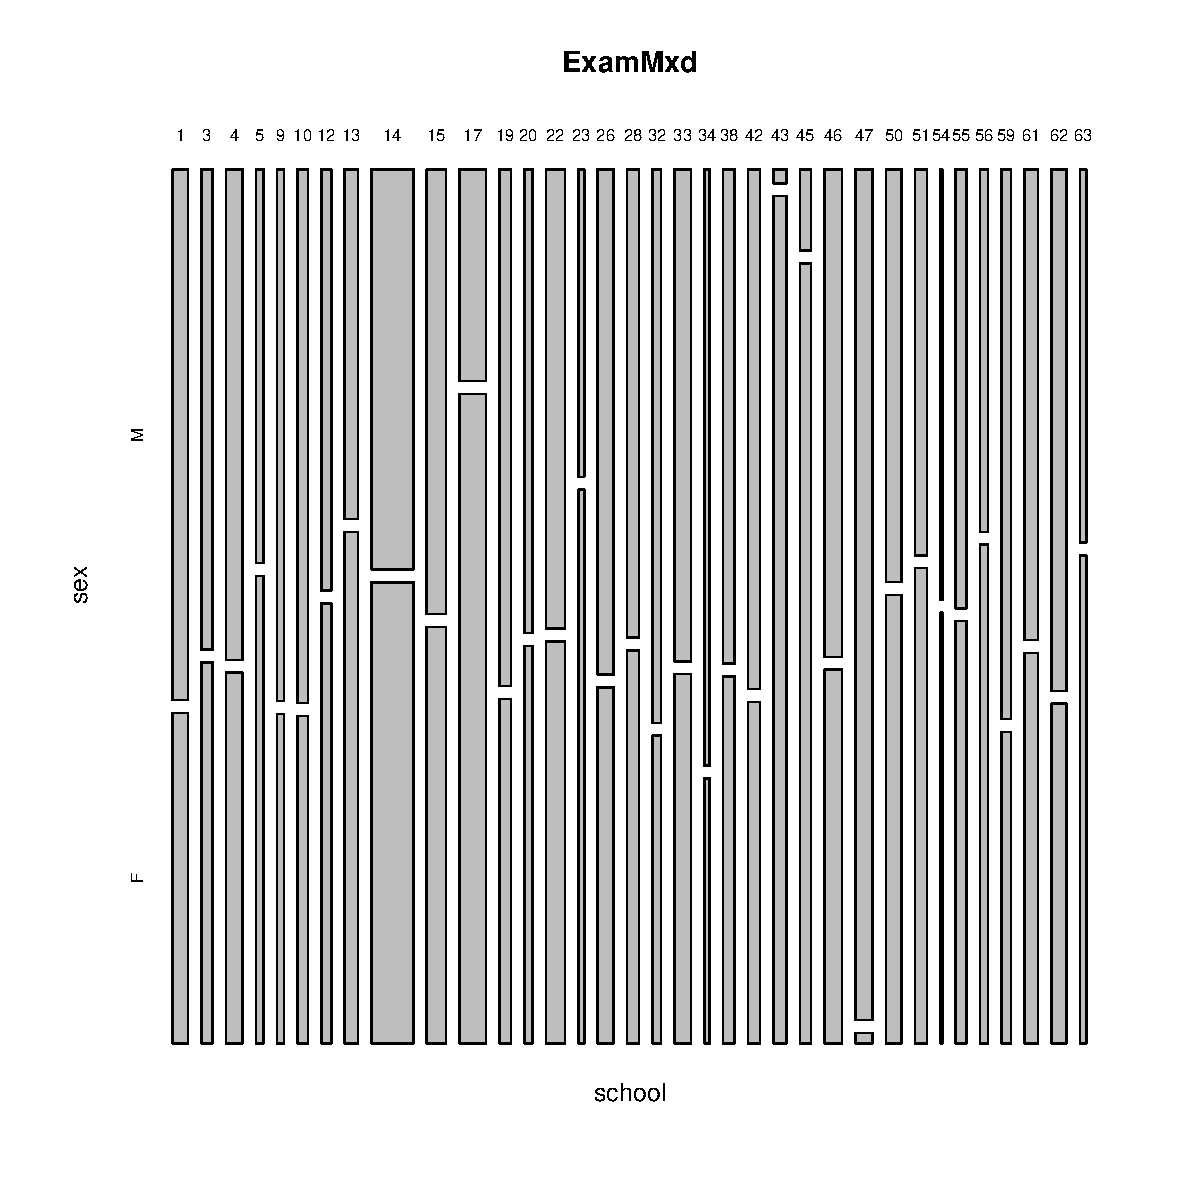
\includegraphics[width=\textwidth]{figs/SoftRev-ExamMosaic}
  \caption{A mosaic plot of the sex distribution by school.  The areas
    of the rectangles are proportional to the number of students of
    that sex from that school who took the exam.  Schools with an
    unusally large or unusually small ratio or females to males are
    highlighted.}
  \label{fig:ExamMosaic}
\end{figure}

\subsubsection{Preliminary graphical displays}
\label{sec:Graphical}

In addition to the pretest score (\code{standLRT}), the predictor
variables used in this model are the student's sex and the school
gender, which is coded as having three levels.  There is some
redundancy in these two variables in that all the students in a
boys-only school must be male.  For graphical exploration we convert
from \code{schgend} to \code{type}, an indicator of whether the school
is a mixed-sex school or a single-sex school, and plot the response
versus the pretest score for each combination of sex and school type.
\begin{figure}[tbp]
  \centering
  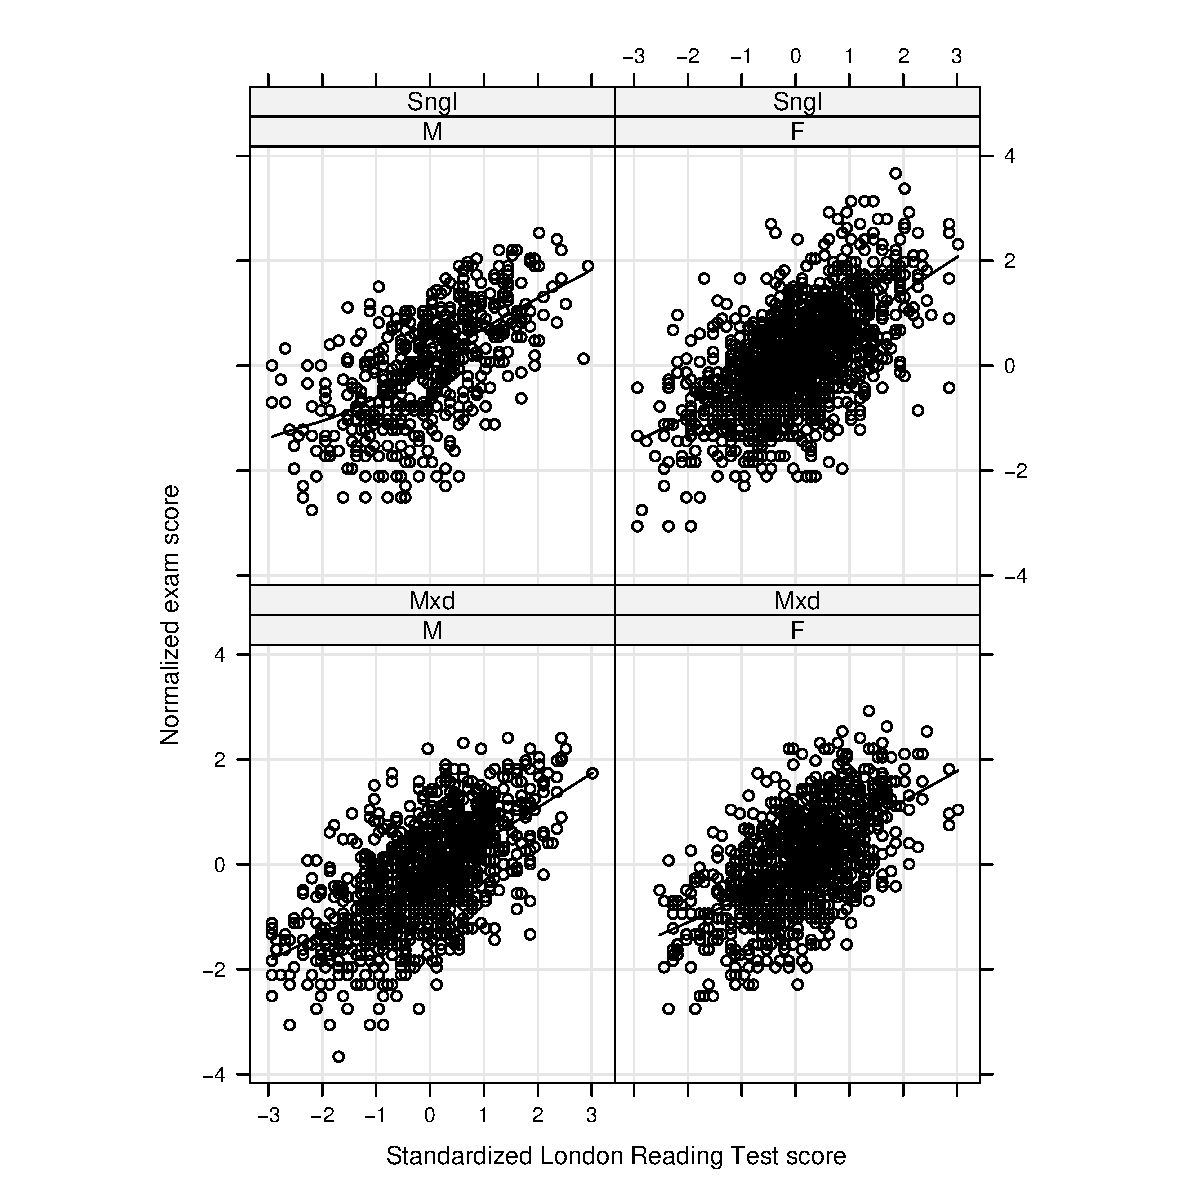
\includegraphics[width=\textwidth]{figs/SoftRev-Examplot1}
  \caption{Normalized exam score versus pretest 
    (Standardized London Reading Test) score for 4095 students from 65 schools
    in inner London. The panels on the left show the male students'
    scores; those on the right show the females' scores.  The top row
    of panels shows the scores of students in single-sex schools and
    the bottom row shows the scores of students in mixed-sex
    schools. A scatterplot smoother line for each panel has been added
    to help visualize the trend.}
  \label{fig:Examplot1}
\end{figure}

This plot is created with the \code{xyplot} from the \code{lattice}
package as (essentially)
\begin{Schunk}
\begin{Sinput}
> xyplot(normexam ~ standLRT | sex * type, Exam, type = c("g", 
+     "p", "smooth"))
\end{Sinput}
\end{Schunk}
The formula would be read as ``plot \code{normexam} by \code{standLRT}
given \code{sex} by (school) \code{type}''.  A few other arguments were
added in the actual call to make the axis annotations more readable.

Figure~\ref{fig:Examplot1} shows the even after accounting for a
student's sex, pretest score and school type, there is considerable
variation in the response.  We may attribute some of this variation to
differences in schools but the fitted model indicates that most of the
variation is unaccounted or ``residual'' variation.

In some ways the high level of residual variation obscures the pattern
in the data.  By removing the data points and overlaying the
scatterplot smoothers we can concentrate on the relationships between
the covariates.
\begin{figure}[tbp]
  \centering
  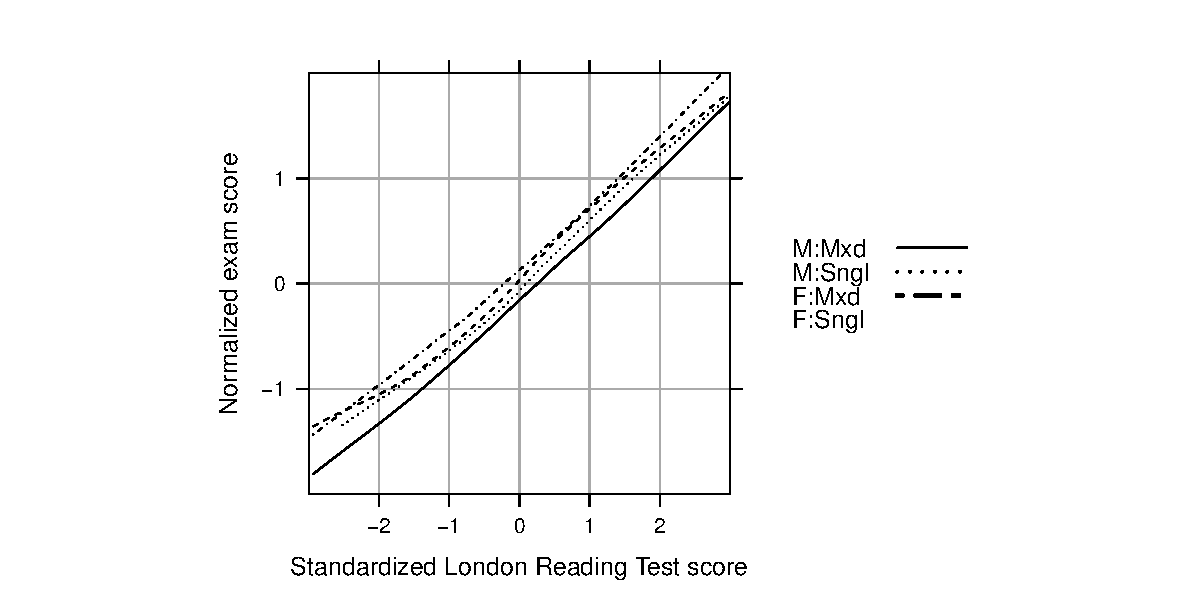
\includegraphics[width=\textwidth]{figs/SoftRev-Examplot2}
  \caption{Overlaid scatterplot smoother lines of the normalized test
    scores versus the pretest (Standardized London Reading Test) score
    for female (F) and male (M) students in single-sex (Sngl) and
    mixed-sex (Mxd) schools.}
  \label{fig:Examplot2}
\end{figure}
The call to \code{xyplot} is essentially
\begin{Schunk}
\begin{Sinput}
> xyplot(normexam ~ standLRT, Exam, groups = sex:type, type = c("g", 
+     "smooth"))
\end{Sinput}
\end{Schunk}

Figure~\ref{fig:Examplot2} is a remarkable plot in that it shows
nearly a perfect ``main effects'' relationship of the response with
the three covariates and almost no interaction.  It is rare to see
real data follow a simple theoretical relationship so closely.

To elaborate, we can see that for each of the four groups the smoothed
relationship between the exam score and the pretest score is close to
a straight line and that the lines are close to being parallel.  The
only substantial deviation is in the smoothed relationship for the
males in single-sex schools and this is the group with the fewest
observations and hence the least precision in the estimated
relationship.  The lack of parallelism for this group is most apparent
in the region of extremely low pretest scores where there are few
observations and a single student who had a low pretest score and a
moderate post-test score can substantially influence the curve.  Five
or six such points can be seen in the upper left panel of
Figure~\ref{fig:Examplot1}. 

We should also notice the ordering of the lines and the spacing
between the lines.  The smoothed relationships for students in
single-sex schools are consistently above those in the mixed-sex
schools and, except for the region of low pretest scores described
above, the relationship for the females in a given type of school is
consistently above that for the males.  Furthermore the distance
between the female and male lines in the single-sex schools is
approximately the same as the corresponding distance in the mixed-sex
schools.  We would summarize this by saying that there is a positive
effect for females versus males and a positive effect for single-sex
versus mixed-sex and no indication of interaction between these
factors.


\subsubsection{The effect of schools}
\label{sec:schoolEffects}

We can check for patterns within and between schools by plotting the
response versus the pretest by school.  Because there appear to be
differences in this relationship for single-sex versus mixed-sex
schools and for females versus males we consider these separately.
\begin{figure}[tbp]
  \centering
  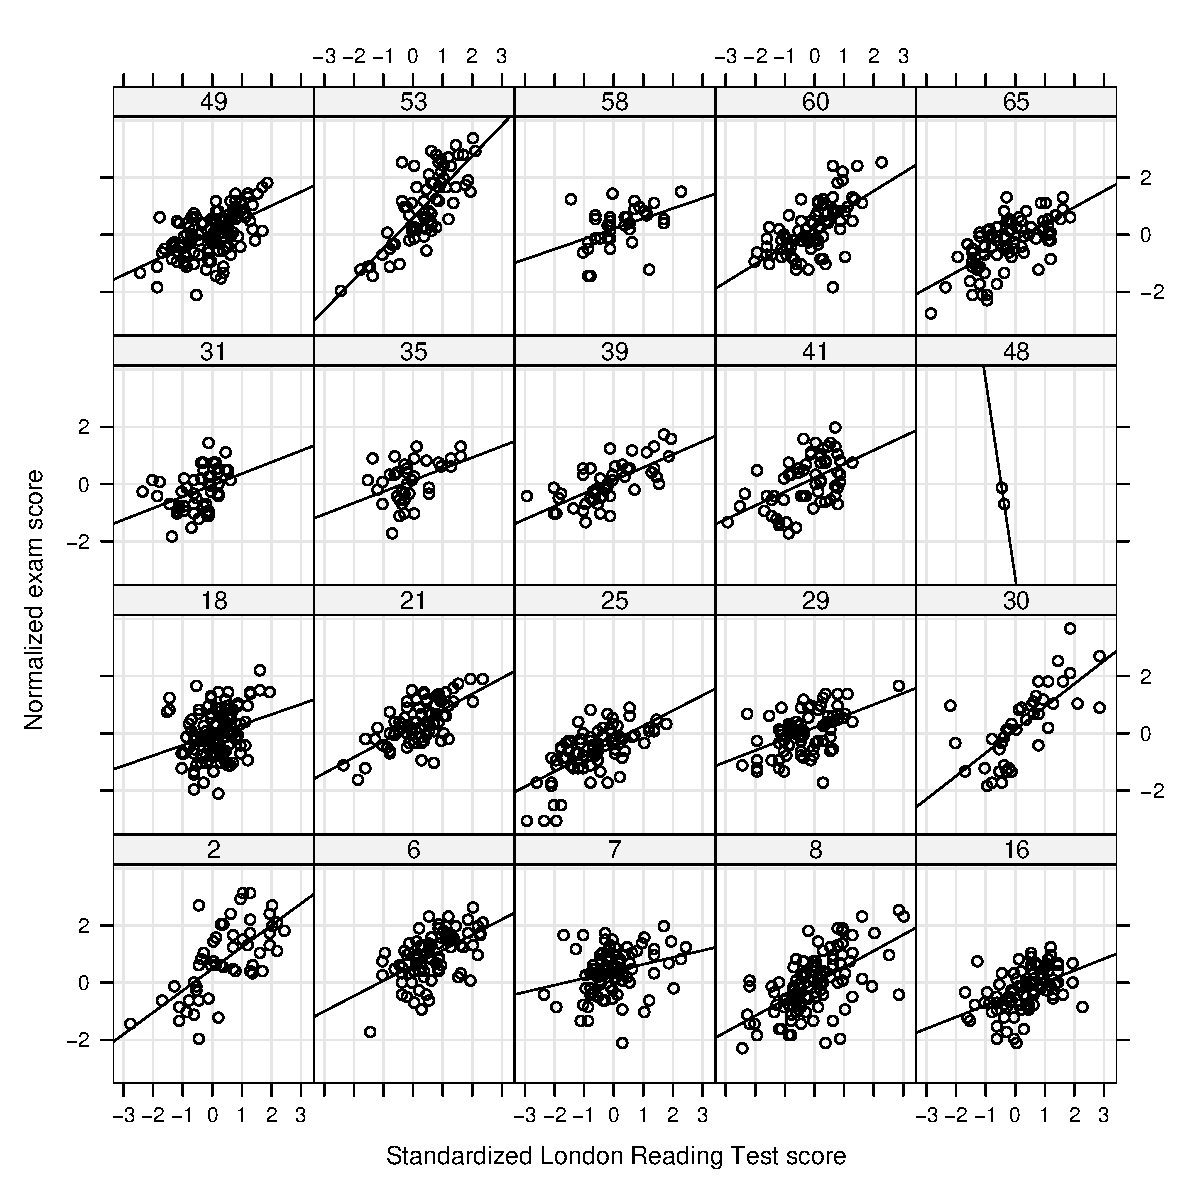
\includegraphics[width=\textwidth]{figs/SoftRev-Examplot3}
  \caption{Normalized exam scores versus pretest (Standardized London
    Reading Test) score by school for female students in single-sex
    schools.}
  \label{fig:Examplot3}
\end{figure}

In Figure~\ref{fig:Examplot3} we plot the normalized exam scores
versus the pretest score by school for female students in single-sex
schools.  The plot is produced as
\begin{Schunk}
\begin{Sinput}
> xyplot(normexam ~ standLRT | school, Exam, type = c("g", "p", 
+     "r"), subset = sex == "F" & type == "Sngl")
\end{Sinput}
\end{Schunk}
The \code{"r"} in the \code{type} argument adds a simple linear
regression line to each panel.

The first thing we notice in Figure~\ref{fig:Examplot3} is that
school 48 is an anomaly because only two students in this school took
the exam.  Because within-school results based on only two students
are unreliable, we will exclude this school from further plots (but we
do include these data when fitting comprehensive models).

Although the regression lines on the panels can help us to look for
variation in the schools, the ordering of the panels is, for our
purposes, random.  We recreate this plot in Figure~\ref{fig:Examplot4} using
\begin{Schunk}
\begin{Sinput}
> xyplot(normexam ~ standLRT | school, Exam, type = c("g", "p", 
+     "r"), subset = sex == "F" & type == "Sngl" & school != 48, 
+     index.cond = function(x, y) coef(lm(y ~ x))[1])
\end{Sinput}
\end{Schunk}
\begin{figure}[tbp]
  \centering
  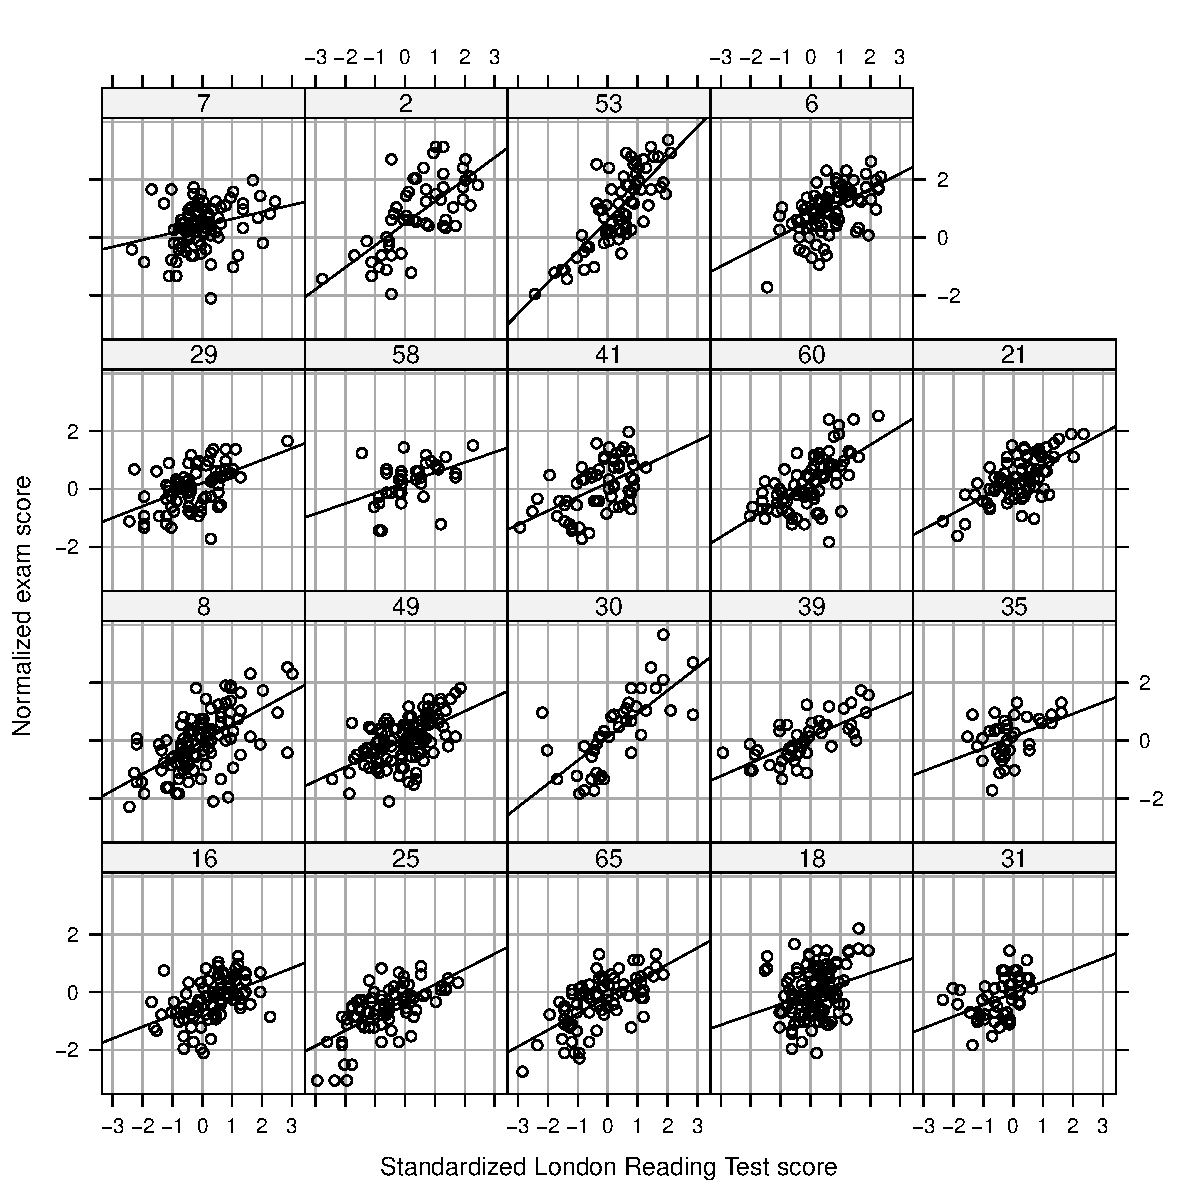
\includegraphics[width=\textwidth]{figs/SoftRev-Examplot4}
  \caption{Normalized exam scores versus pretest (Standardized London
    Reading Test) score by school for female students in single-sex
    schools. School 48 where only two students took the exam has been
    eliminated and the panels have been ordered by increasing
    intercept (predicted normalized score for a pretest score of 0) of
    the regression line.}
  \label{fig:Examplot4}
\end{figure}
so that the panels are ordered (from left to right starting at the
bottom row) by increasing intercept for the regression line (i.e.{} by
increasing predicted exam score for a student with a pretest score of 0).

Alternatively, we could order the panels by increasing slope of the
within-school regression lines, as in Figure~\ref{fig:Examplot4a}.
\begin{figure}[tbp]
  \centering
  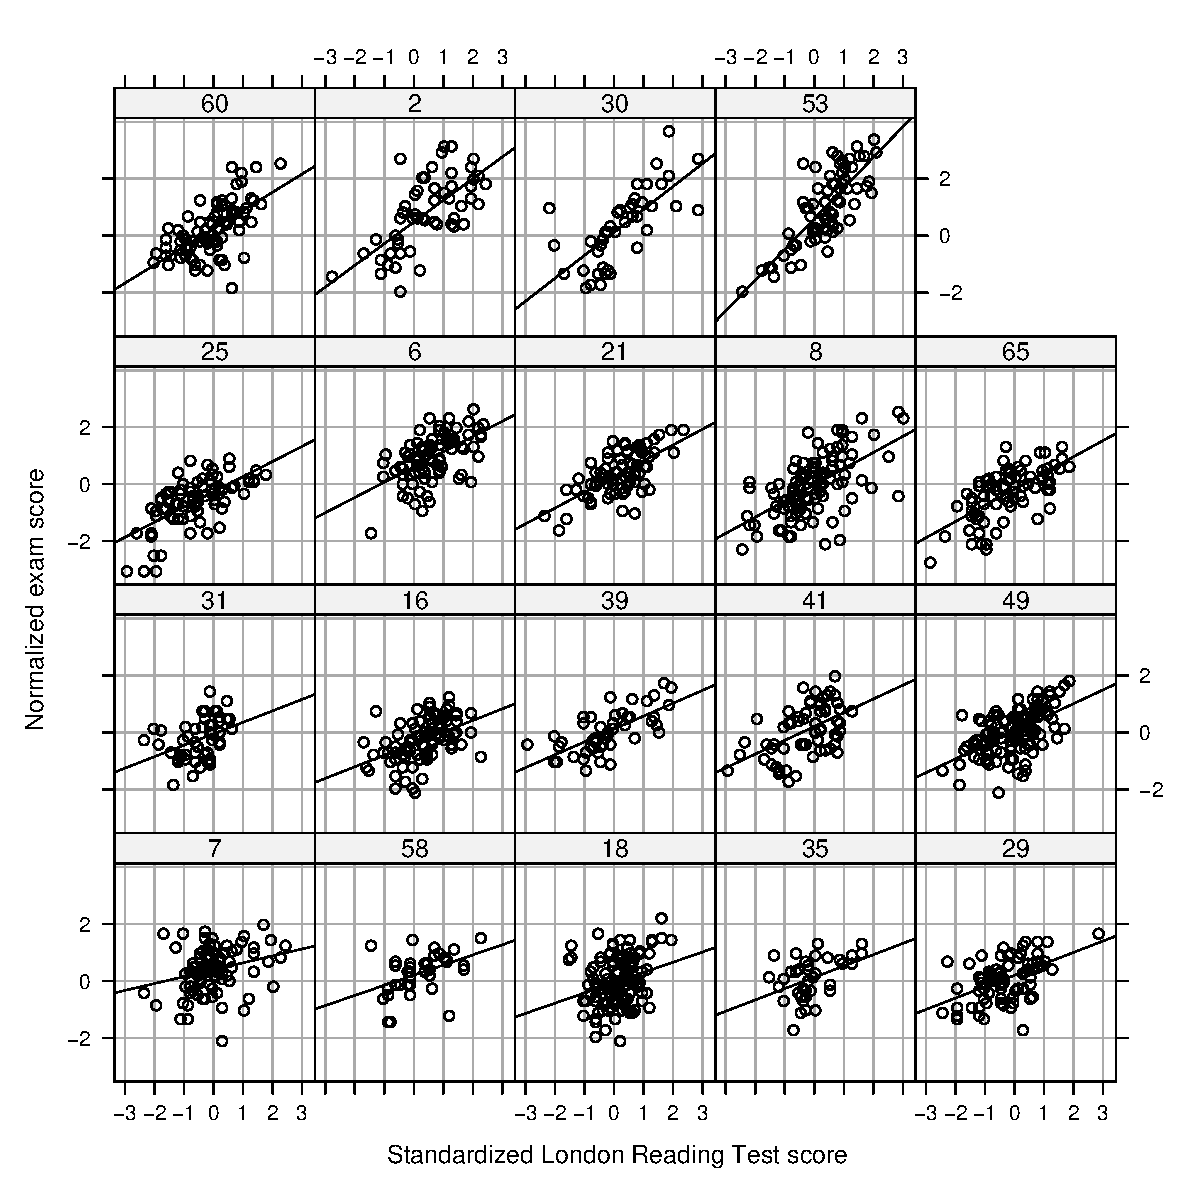
\includegraphics[width=\textwidth]{figs/SoftRev-Examplot4a}
  \caption{Normalized exam scores versus pretest (Standardized London
    Reading Test) score by school for female students in single-sex
    schools. School 48 has been eliminated and the panels have been
    ordered by increasing slope of the within-school regression
    lines.}
  \label{fig:Examplot4a}
\end{figure}

Although it is informative to plot the within-school regression lines
we need to assess the variability in the estimates of the coefficients
before concluding if there is ``significant'' variability between
schools.  We can obtain the individual regression fits with the
\code{lmList} function
\begin{Schunk}
\begin{Sinput}
> show(ExamFS <- lmList(normexam ~ standLRT | school, Exam, subset = sex == 
+     "F" & type == "Sngl" & school != 48))
\end{Sinput}
\begin{Soutput}
Call: lmList(formula = normexam ~ standLRT | school, data = Exam, subset = sex ==      "F" & type == "Sngl" & school != 48) 
Coefficients:
   (Intercept)  standLRT
2   0.48227991 0.7612884
6   0.60321439 0.5353444
7   0.39852689 0.2422785
8  -0.02519463 0.5674053
16 -0.38564292 0.4069399
18 -0.05733995 0.3593830
21  0.26872018 0.5544939
25 -0.26779146 0.5320575
29  0.20442314 0.4005158
30  0.11885028 0.8059021
31 -0.03922548 0.4022838
35  0.13173022 0.3966535
39  0.12754208 0.4525918
41  0.21249712 0.4834107
49  0.04747055 0.4845568
53  0.59370349 1.0769781
58  0.20707724 0.3557839
60  0.25196603 0.6378090
65 -0.17490019 0.5684592

Degrees of freedom: 1375 total; 1337 residual
Residual standard error: 0.7329521
\end{Soutput}
\end{Schunk}
and compare the confidence intervals on these coefficients.
\begin{Schunk}
\begin{Sinput}
> plot(confint(ExamFS, pool = TRUE), order = 1)
\end{Sinput}
\end{Schunk}
\begin{figure}[tbp]
  \centering
  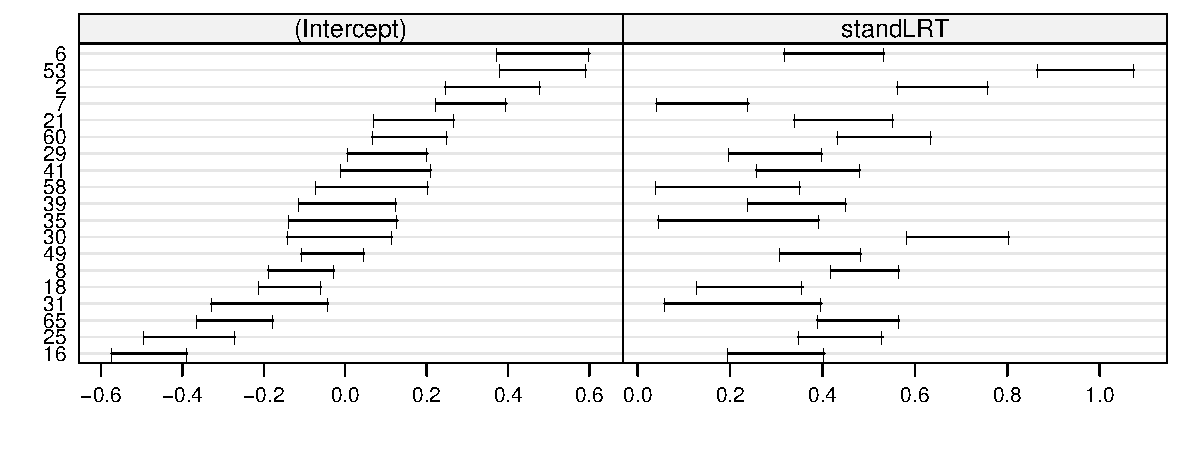
\includegraphics[width=\textwidth]{figs/SoftRev-Examplot4c}
  \caption{Confidence intervals on the coefficients of the
    within-school regression lines for female students in single-sex
    schools. School 48 has been eliminated and the schools have been
    ordered by increasing estimated intercept.}
  \label{fig:Examplot4c}
\end{figure}


\begin{figure}[tbp]
  \centering
  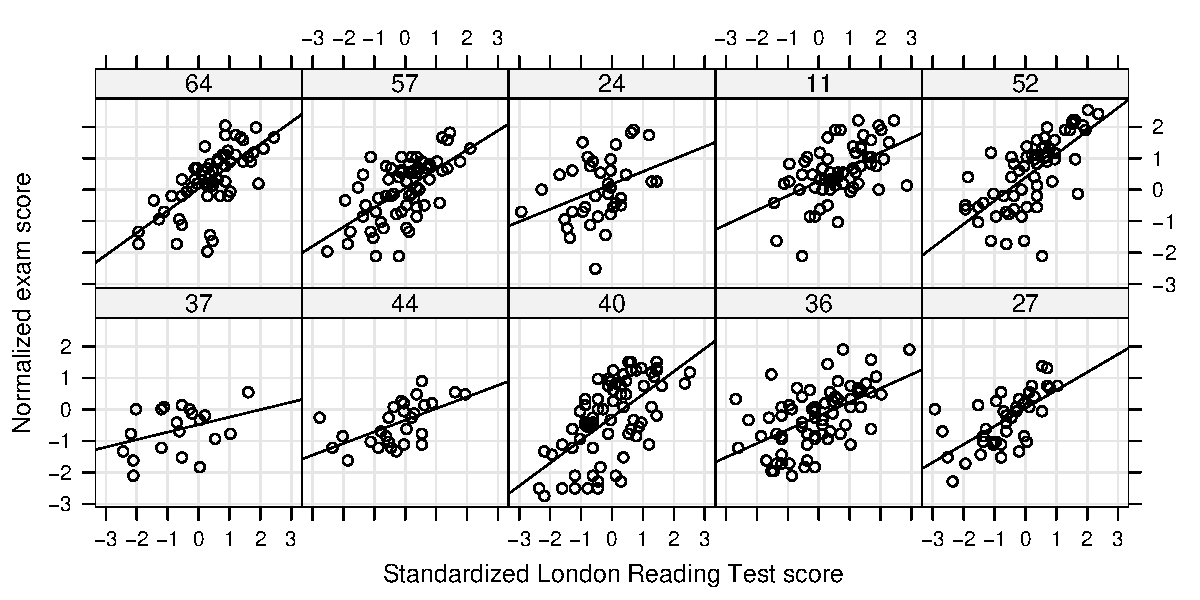
\includegraphics[width=\textwidth]{figs/SoftRev-Examplot5}
  \caption{Normalized exam scores versus pretest (Standardized London
    Reading Test) score by school for male students in single-sex
    schools.}
  \label{fig:Examplot5}
\end{figure}

\begin{Schunk}
\begin{Sinput}
> show(ExamMS <- lmList(normexam ~ standLRT | school, Exam, subset = sex == 
+     "M" & type == "Sngl"))
\end{Sinput}
\begin{Soutput}
Call: lmList(formula = normexam ~ standLRT | school, data = Exam, subset = sex ==      "M" & type == "Sngl") 
Coefficients:
   (Intercept)  standLRT
11  0.26596312 0.4586355
24  0.17773174 0.3976156
27  0.03518861 0.5728684
36 -0.20691842 0.4383453
37 -0.48522245 0.2382739
40 -0.25019842 0.7262845
44 -0.34440523 0.3696269
52  0.38803903 0.7402692
57  0.04055154 0.6123692
64  0.03749455 0.7055239

Degrees of freedom: 513 total; 493 residual
Residual standard error: 0.8082068
\end{Soutput}
\end{Schunk}
The corresponding plot of the confidence intervals is shown in
Figure~\ref{fig:Examplot5b}.
\begin{figure}[tbp]
  \centering
  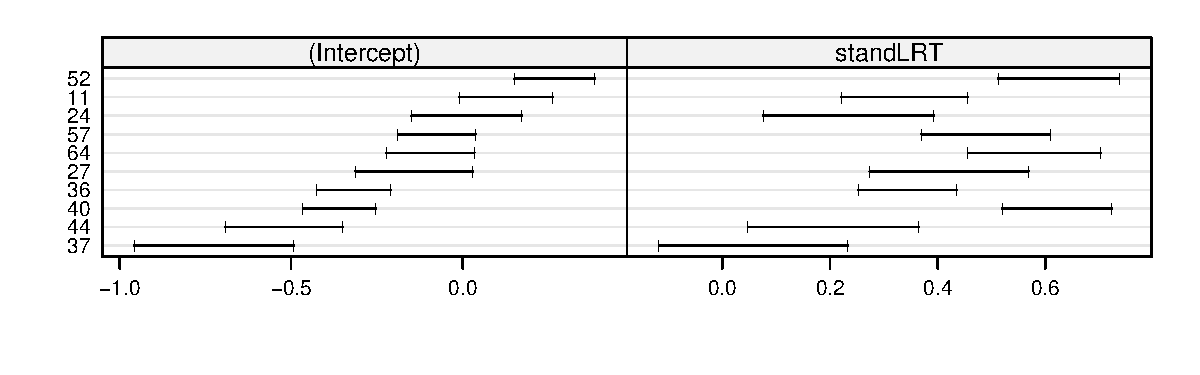
\includegraphics[width=\textwidth]{figs/SoftRev-Examplot5b}
  \caption{Confidence intervals on the coefficients of the
    within-school regression lines for female students in single-sex
    schools. School 48 has been eliminated and the schools have been
    ordered by increasing estimated intercept.}
  \label{fig:Examplot5b}
\end{figure}

For the mixed-sex schools we can consider the effect of the pretest
score and sex in the plot (Figure~\ref{fig:Examplot6}) and in the
\begin{figure}[tbp]
  \centering
  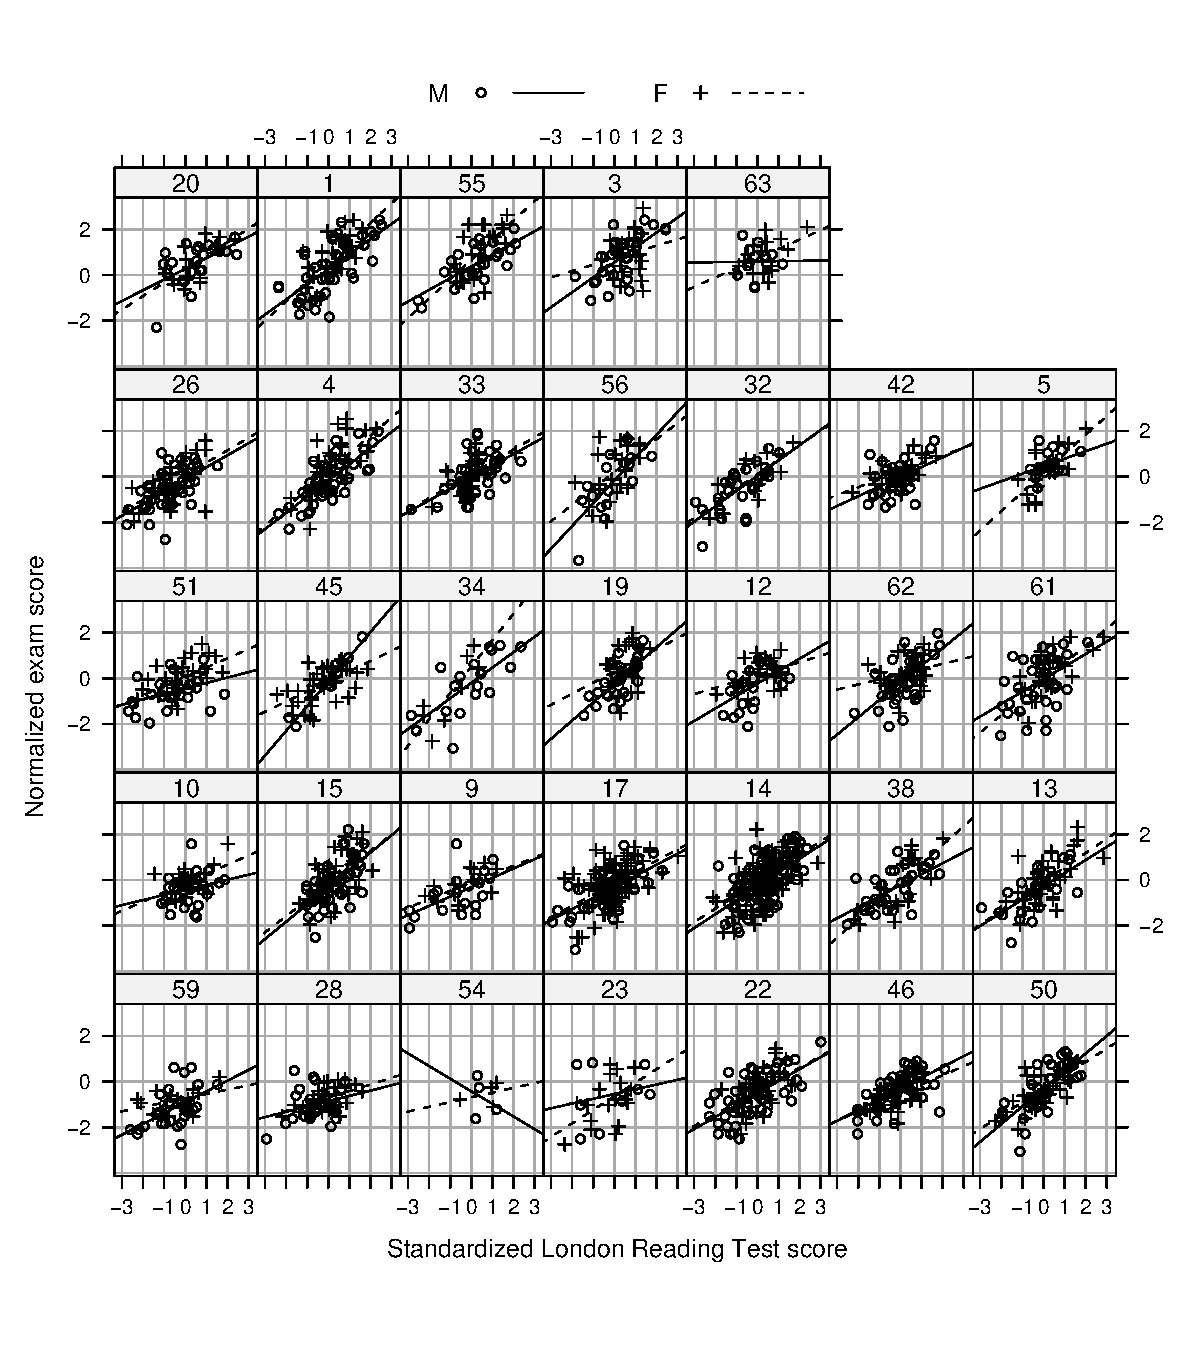
\includegraphics[width=\textwidth]{figs/SoftRev-Examplot6}
  \caption{Normalized exam scores versus pretest
    score by school and sex for students in mixed-sex
    schools.}
  \label{fig:Examplot6}
\end{figure}
separate model fits for each school.
\begin{Schunk}
\begin{Sinput}
> show(ExamM <- lmList(normexam ~ standLRT + sex | school, Exam, 
+     subset = type == "Mxd" & !school %in% c(43, 47, 54)))
\end{Sinput}
\begin{Soutput}
Call: lmList(formula = normexam ~ standLRT + sex | school, data = Exam,      subset = type == "Mxd" & !school %in% c(43, 47, 54)) 
Coefficients:
   (Intercept)  standLRT         sexF
1   0.24770238 0.7044798  0.355719842
3   0.58030950 0.5843480 -0.057223931
4  -0.16739321 0.7372405  0.402829332
5   0.36213174 0.6695127 -0.183238345
9  -0.32487665 0.3961812  0.222382659
10 -0.45139239 0.2972074  0.330917735
12 -0.26201220 0.4200265  0.378359201
13 -0.27196976 0.6037392  0.196013604
14 -0.28741229 0.5966633  0.202122649
15 -0.30963145 0.7370363  0.144392527
17 -0.30553035 0.4905235  0.156646395
19 -0.22542808 0.7214611  0.385544198
20  0.25120209 0.5187894  0.041342515
22 -0.50744197 0.5206371  0.089368918
23 -0.51727825 0.3873051 -0.189332381
26 -0.11870804 0.5342909  0.185283146
28 -0.84451962 0.2583861  0.138672637
32  0.02596084 0.6560569  0.082029123
33 -0.02539396 0.5148927  0.147967544
34 -0.19582273 0.7662681  0.327656212
38 -0.19255275 0.6184554  0.084872081
42 -0.01913469 0.3827088  0.246533297
45 -0.21212351 0.5665400  0.102317128
46 -0.30554555 0.4491187 -0.201294993
50 -0.32718434 0.6752947  0.001906973
51 -0.40150931 0.3076539  0.445100548
55  0.35743002 0.6118447  0.400034477
56 -0.18744293 0.8558783  0.391178135
59 -0.97233088 0.3594417  0.329480168
61 -0.01215078 0.6428683 -0.060024560
62 -0.16445110 0.5411566  0.283642476
63  0.60216184 0.3091657  0.150390337

Degrees of freedom: 2018 total; 1922 residual
Residual standard error: 0.7273955
\end{Soutput}
\end{Schunk}
The confidence intervals for these separately fitted models, 
\begin{figure}[tbp]
  \centering
  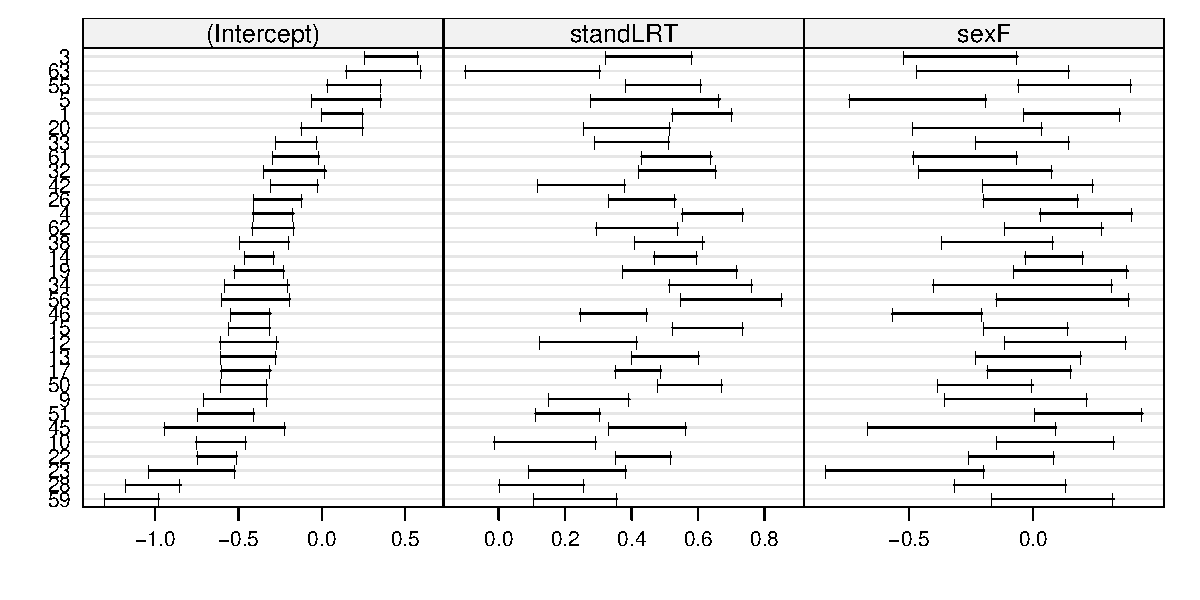
\includegraphics[width=\textwidth]{figs/SoftRev-Examplot6b}
  \caption{Confidence intervals on the coefficients of the
    within-school regression lines for female students in single-sex
    schools. School 48 has been eliminated and the schools have been
    ordered by increasing estimated intercept.}
  \label{fig:Examplot6b}
\end{figure}
shown in Figure~\ref{fig:Examplot6b} indicate differences in the
intercepts and possibly differences in the slopes with respect to the
pretest scores.  However, there is not a strong indication of
variation by school in the effect of sex.


\subsection{Multilevel models for the exam data}
\label{sec:ExamModels}

We begin with a model that has a random effects for the intercept by
school plus additive fixed effects for the pretest score, the
student's sex and the school type.
\begin{Schunk}
\begin{Sinput}
> (Em3 <- lmer(normexam ~ standLRT + sex + type + (1 | school), 
+     Exam))
\end{Sinput}
\begin{Soutput}
Linear mixed-effects model fit by REML
Formula: normexam ~ standLRT + sex + type + (1 | school) 
   Data: Exam 
      AIC      BIC    logLik MLdeviance REMLdeviance
 9357.384 9395.237 -4672.692   9325.485     9345.384
Random effects:
 Groups   Name        Variance Std.Dev.
 school   (Intercept) 0.084367 0.29046 
 Residual             0.562529 0.75002 
# of obs: 4059, groups: school, 65

Fixed effects:
               Estimate  Std. Error   DF t value  Pr(>|t|)
(Intercept)   -0.167682    0.054680 4055 -3.0666  0.002179
standLRT       0.559834    0.012448 4055 44.9725 < 2.2e-16
sexF           0.165959    0.032812 4055  5.0579 4.426e-07
typeSngl       0.165458    0.077428 4055  2.1369  0.032663
\end{Soutput}
\end{Schunk}
Our data exploration indicated that the slope with respect to the
pretest score may vary by school.  We can fit a model with random
effects by school for both the slope and the intercept as
\begin{Schunk}
\begin{Sinput}
> (Em4 <- lmer(normexam ~ standLRT + sex + type + (standLRT | school), 
+     Exam))
\end{Sinput}
\begin{Soutput}
Linear mixed-effects model fit by REML
Formula: normexam ~ standLRT + sex + type + (standLRT | school) 
   Data: Exam 
      AIC      BIC    logLik MLdeviance REMLdeviance
 9316.573 9367.043 -4650.287    9281.17     9300.573
Random effects:
 Groups   Name        Variance Std.Dev. Corr  
 school   (Intercept) 0.082477 0.28719        
          standLRT    0.015081 0.12280  0.579 
 Residual             0.550289 0.74181        
# of obs: 4059, groups: school, 65

Fixed effects:
               Estimate  Std. Error   DF t value  Pr(>|t|)
(Intercept)   -0.188698    0.051940 4055 -3.6330 0.0002836
standLRT       0.554101    0.020117 4055 27.5433 < 2.2e-16
sexF           0.167971    0.032281 4055  5.2034 2.054e-07
typeSngl       0.176390    0.069587 4055  2.5348 0.0112876
\end{Soutput}
\end{Schunk}
and compare this fit to the previous fit with
\begin{Schunk}
\begin{Sinput}
> anova(Em3, Em4)
\end{Sinput}
\begin{Soutput}
Data: Exam
Models:
Em3: normexam ~ standLRT + sex + type + (1 | school)
Em4: normexam ~ standLRT + sex + type + (standLRT | school)
    Df     AIC     BIC  logLik  Chisq Chi Df Pr(>Chisq)
Em3  6  9357.4  9395.2 -4672.7                         
Em4  8  9316.6  9367.0 -4650.3 44.811      2  1.859e-10
\end{Soutput}
\end{Schunk}
There is a strong evidence of a significant random effect for the
slope by school, whether judged by AIC, BIC or the p-value for the
likelihood ratio test.

The p-value for the likelihood ratio test is based on a $\chi^2$ distribution
with degrees of freedom calculated as the difference in the number of
parameters in the two models.  Because one of the parameters
eliminated from the full model in the submodel is at its boundary the
usual asymptotics for the likelihood ratio test do not apply.
However, it can be shown that the p-value quoted for the test is
conservative in the sense that it is an upper bound on the 
p-value that would be calculated say from a parametric bootstrap.

Having an upper bound of $1.9\times 10^{-10}$ on the p-value can be
regarded as ``highly significant'' evidence of the utility of the
random effect for the slope by school.

We could also add a random effect for the student's sex by school
\begin{Schunk}
\begin{Sinput}
> (Em5 <- lmer(normexam ~ standLRT + sex + type + (standLRT + sex | 
+     school), Exam))
\end{Sinput}
\begin{Soutput}
Linear mixed-effects model fit by REML
Formula: normexam ~ standLRT + sex + type + (standLRT + sex | school) 
   Data: Exam 
      AIC      BIC    logLik MLdeviance REMLdeviance
 9322.573 9391.969 -4650.287    9281.17     9300.573
Random effects:
 Groups   Name        Variance   Std.Dev.   Corr        
 school   (Intercept) 8.2477e-02 2.8719e-01             
          standLRT    1.5081e-02 1.2281e-01 0.579       
          sexF        2.7514e-10 1.6587e-05 0.000 0.000 
 Residual             5.5029e-01 7.4181e-01             
# of obs: 4059, groups: school, 65

Fixed effects:
               Estimate  Std. Error   DF t value  Pr(>|t|)
(Intercept)   -0.188698    0.051940 4055 -3.6330 0.0002836
standLRT       0.554101    0.020118 4055 27.5431 < 2.2e-16
sexF           0.167971    0.032281 4055  5.2034 2.054e-07
typeSngl       0.176390    0.069587 4055  2.5348 0.0112878
\end{Soutput}
\end{Schunk}
Notice that the estimate of the variance of the \code{sexM} term is
essentially zero so there is no need to test the significance of this
variance component.  We proceed with the analysis of \code{Em4}.


\subsection{Markov Chain Monte Carlo methods for assessing parameter variation}
\label{sec:MCMC}

An important part of the analysis of a statistical model is the
assessment of the precision of parameter estimates, either through
confidence intervals and confidence regions or through hypothesis
tests on the parameters.  Sometimes such information is condensed and
given as the parameter estimate and a standard error of the estimate,
with the assumption that a confidence interval will be formed as the
estimate plus/minus some multiple of the standard error.

Summarizing the variability in parameter estimates with such symmetric
intervals is appropriate if the distribution of the parameters can
be assumed to be reasonably symmetric but this is not the case for
variance components.  In general we expect the distribution of a
variance component to be approximately $\chi^2$ and, depending upon the
precision with which the component is estimated, such a distribution
can be quite asymmetric.

To examine the distribution of the parameter estimates we can use a
parametric bootstrap or adopt a Bayesian approach and generate a
sample from the posterior distribution of the parameters using a
technique called Markov Chain Monte Carlo sampling. The
\code{mcmcsamp} function applied to a fitted \code{lmer} model
generates such a sample.

\begin{Schunk}
\begin{Sinput}
> Es4 <- mcmcsamp(Em4, 10000, trans = FALSE)
\end{Sinput}
\end{Schunk}

The parameter estimates in this sample are the fixed effects, the
variance of the random per-observation noise, $\sigma^2$, the variance
of the intercept random effect, the variance of the slope random
effect and their covariance.  A plot of the estimated posterior
densities of each of the parameters (Figure~\ref{fig:Examplot7})
\begin{figure}[tbp]
  \centering
  \includegraphics[width=\textwidth]{figs/SoftRev-Examplot7}
  \caption{Plots of the estimated posterior probability densities from
    a Markov Chain Monte Carlo sample of the parameters in the model
    \code{Em4}.} 
  \label{fig:Examplot7}
\end{figure}
shows that the posterior densities of the fixed effects are indeed
quite symmetric and close to a normal (or Gaussian) distribution.  The
posterior density of $\sigma^2$ and the covariance parameter are
reasonably symmetric but the posterior densities of the variances of
the random effects are not.

A better way of assessing possible asymmetry is to use normal
probability plots of the samples from each of the parameters, as in
Figure~\ref{fig:Examplot8}.
\begin{figure}[tbp]
  \centering
  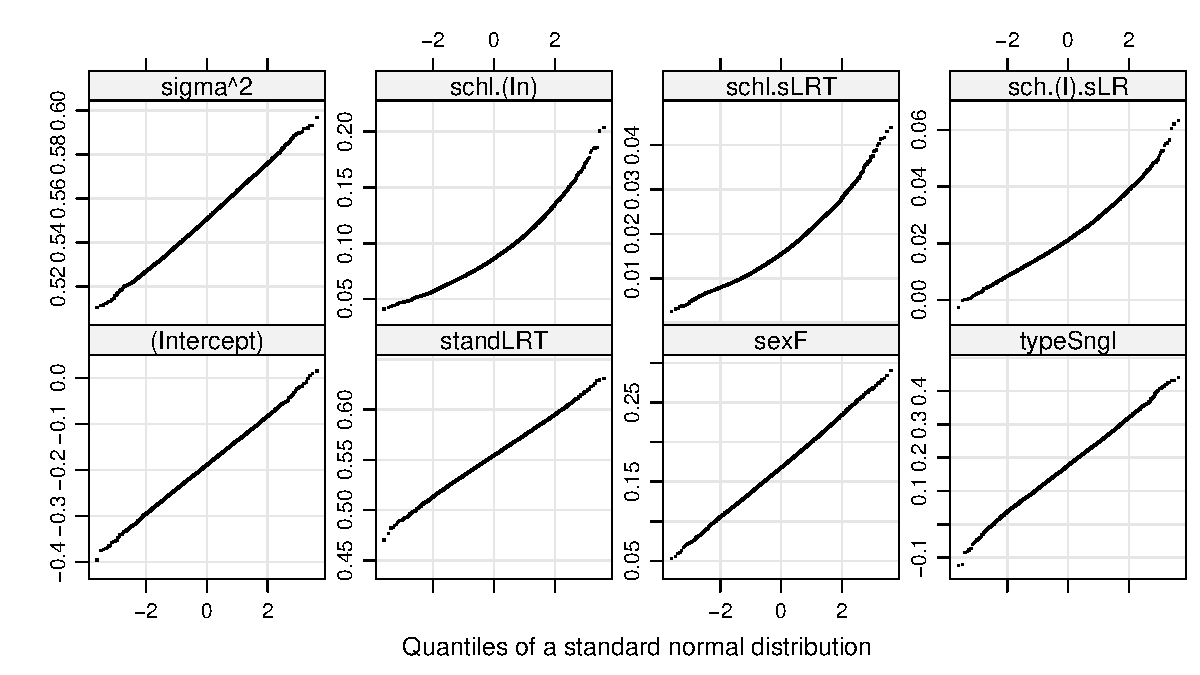
\includegraphics[width=\textwidth]{figs/SoftRev-Examplot8}
  \caption{Normal probability plots of the Markov Chain Monte Carlo
    samples from the posterior densities of the parameters in the
    model \code{Em4}.} 
  \label{fig:Examplot8}
\end{figure}

We can see from Figure~\ref{fig:Examplot8} that the posterior
distributions of the fixed effects are remarkably close to the normal
(or Gaussian) distribution.  Except for a few points in each panel,
these panels show almost perfect linearity.  The few points that do
deviate from the straight line in each case represent fewer than
a dozen samples out of a total of 10,000 and are not a cause for concern.

The posterior distribution of $\sigma^2$ is satisfactorily close to a
normal distribution.  As we will see, it is not always the case that
this parameter is close to normally distributed.  It happens that in
this example $\sigma^2$ is very precisely determined and possible
asymmetry in the distribution will not be noticeable over such a small
range of values.

There is noticeable asymmetry in the distribution of the variances of
the random effects and perhaps some asymmetry in the distribution of
the covariance of the intercept and slope random effects.

Using this sample we can examine the distribution of functions of
these parameters.  For example, \citep{box73:_bayes_infer_statis_analy} advocate
approximating the distribution of the logarithm of a variance rather
than the variance itself.  For a covariance we first convert it to a
correlation then apply Fisher's z transformation (the hyperbolic
arc-tangent) to the correlation.  The density plots and normal
probability plots of these transformed parameters are shown in
Figures~\ref{fig:Examplot9} and \ref{fig:Examplot10}.

\begin{figure}[tbp]
  \centering
  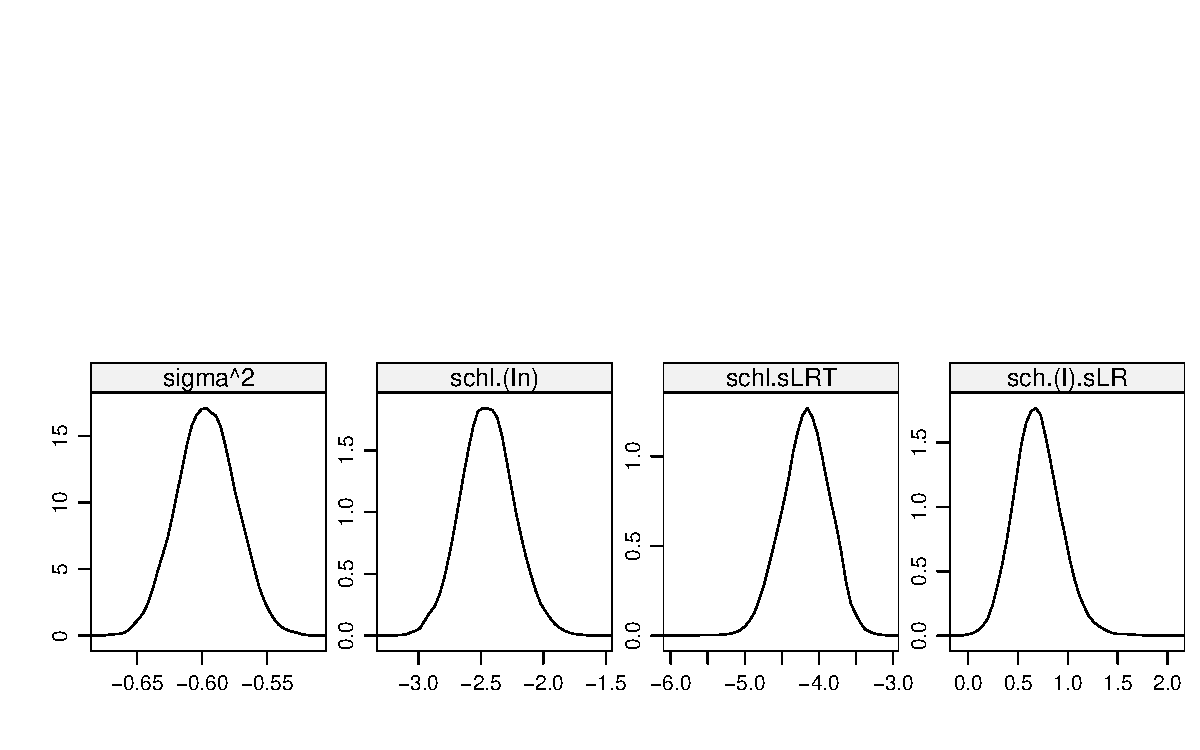
\includegraphics[width=\textwidth]{figs/SoftRev-Examplot9}
  \caption{Estimated density plots of the Markov Chain Monte Carlo
    samples from the posterior densities of the variance and
    covariance parameters in model \code{Em4}.  The variance
    parameters are on the log scale and the covariance is expressed as
    Fisher's z transformation of the correlation.}
  \label{fig:Examplot9}
\end{figure}

\begin{figure}[tbp]
  \centering
  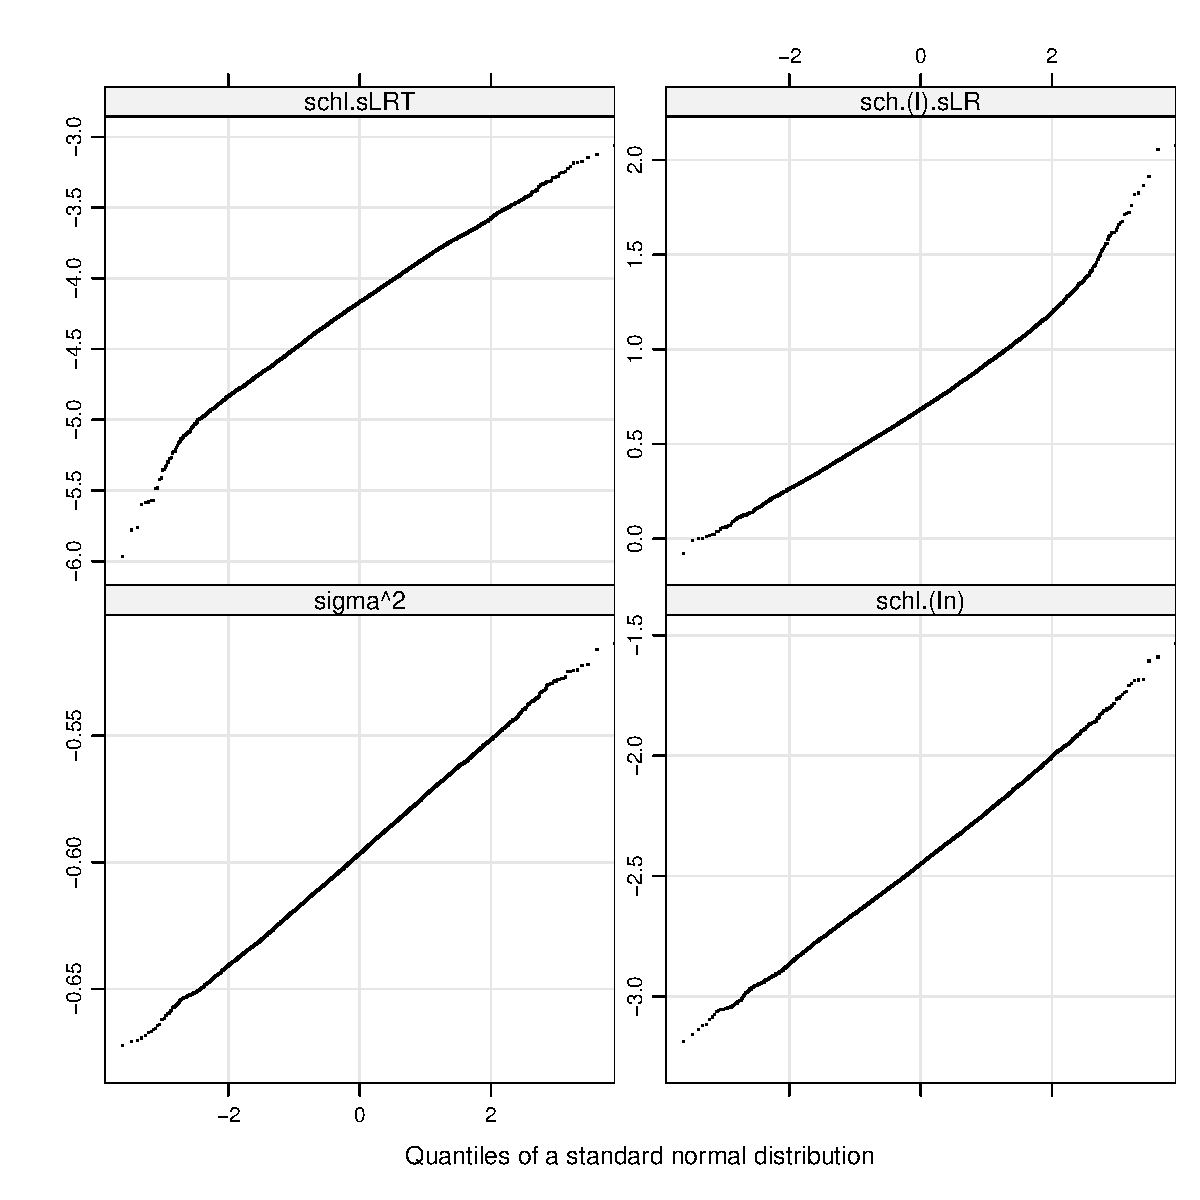
\includegraphics[width=\textwidth]{figs/SoftRev-Examplot10}
  \caption{Normal probability plots of the Markov Chain Monte Carlo
    samples from the posterior densities of the variance and
    covariance parameters in model \code{Em4}.  The variance
    parameters are on the log scale and the covariance is expressed as
    Fisher's z transformation of the correlation.}
  \label{fig:Examplot10}
\end{figure}



\section{Three-level Normal Models}
\label{sec:three-level}

These results are from the 1997 A-level Chemistry exam.  The
\code{school} is nested in \code{lea} (local education authority) and
has unique levels for each of the 2410 schools.  It is a good practice
to make the nesting explicit by specifying the grouping factors as the
`outer' factor, \code{lea} in this case, and the interaction of the
outer and inner factors, \code{lea:school} or \code{school:lea} in
this case.  This will ensure unique levels for each \code{school}
within \code{lea} combination.

To fit the model \code{mC2} we increase the number of EM iterations
from its default of 20 to 40.  Without this change the current version
of the \code{optim} function in \RR{} will declare convergence to an
incorrect optimum.  By increasing the number of EM iterations we are
able to get closer to the optimum before calling \code{optim} and
converge to the correct value.  The optim function will be patched so
this change will not be needed in future versions of \RR{}.

Data from the 1997 A-level Chemistry exam are available as \code{Chem97}.

\begin{Schunk}
\begin{Sinput}
> str(Chem97)
\end{Sinput}
\begin{Soutput}
`data.frame':	31022 obs. of  8 variables:
 $ lea      : Factor w/ 131 levels "1","2","3","4",..: 1 1 1 1 1 1 1 1 1 1 ...
 $ school   : Factor w/ 2410 levels "1","2","3","4",..: 1 1 1 1 1 1 1 1 1 1 ...
 $ student  : Factor w/ 31022 levels "1","2","3","4",..: 1 2 3 4 5 6 7 8 9 10 ...
 $ score    : num  4 10 10 10 8 10 6 8 4 10 ...
 $ gender   : Factor w/ 2 levels "M","F": 2 2 2 2 2 2 2 2 2 2 ...
 $ age      : num  3 -3 -4 -2 -1 4 1 4 3 0 ...
 $ gcsescore: num  6.62 7.62 7.25 7.50 6.44 ...
 $ gcsecnt  : num  0.339 1.339 0.964 1.214 0.158 ...
\end{Soutput}
\begin{Sinput}
> system.time(mC1 <- lmer(score ~ 1 + (1 | lea:school) + (1 | lea), 
+     Chem97), gc = TRUE)
\end{Sinput}
\begin{Soutput}
[1] 2.90 0.11 3.00 0.00 0.00
\end{Soutput}
\begin{Sinput}
> summary(mC1)
\end{Sinput}
\begin{Soutput}
Linear mixed-effects model fit by REML
Formula: score ~ 1 + (1 | lea:school) + (1 | lea) 
   Data: Chem97 
      AIC      BIC   logLik MLdeviance REMLdeviance
 157881.8 157915.2 -78936.9   157869.9     157873.8
Random effects:
 Groups     Name        Variance Std.Dev.
 lea:school (Intercept) 2.74878  1.6579  
 lea        (Intercept) 0.15351  0.3918  
 Residual               8.51607  2.9182  
# of obs: 31022, groups: lea:school, 2410; lea, 131

Fixed effects:
              Estimate Std. Error    DF t value  Pr(>|t|)
(Intercept) 5.3190e+00 5.8110e-02 31021  91.533 < 2.2e-16
\end{Soutput}
\begin{Sinput}
> system.time(mC2 <- lmer(score ~ gcsecnt + (1 | school) + (1 | 
+     lea), Chem97, control = list(niterEM = 40)), gc = TRUE)
\end{Sinput}
\begin{Soutput}
[1] 0.90 0.03 0.93 0.00 0.00
\end{Soutput}
\begin{Sinput}
> summary(mC2)
\end{Sinput}
\begin{Soutput}
Linear mixed-effects model fit by REML
Formula: score ~ gcsecnt + (1 | school) + (1 | lea) 
   Data: Chem97 
    AIC      BIC   logLik MLdeviance REMLdeviance
 141707 141748.7 -70848.5   141685.6       141697
Random effects:
 Groups   Name        Variance Std.Dev.
 school   (Intercept) 1.166190 1.07990 
 lea      (Intercept) 0.014754 0.12147 
 Residual             5.154206 2.27029 
# of obs: 31022, groups: school, 2410; lea, 131

Fixed effects:
              Estimate Std. Error    DF t value  Pr(>|t|)
(Intercept) 5.6355e+00 3.1232e-02 31020  180.44 < 2.2e-16
gcsecnt     2.4726e+00 1.6904e-02 31020  146.27 < 2.2e-16

Correlation of Fixed Effects:
        (Intr)
gcsecnt 0.058 
\end{Soutput}
\end{Schunk}


\section{Two-level models for binary data}
\label{sec:TwolevelBinary}

When the response variable is binary or when it represents a count we
frequently model the data with a \emph{generalized linear model} (glm)
or, if we use random effects in the model, a \emph{generalized linear
  mixed model} (glmm).  Determining maximum likelihood estimates of
the parameters in such a model is not as easy as for the linear mixed
model because the likelihood for a glmm is expressed as an integral
that must be approximated. 

The \code{lmer} function has provision for fitting such models using
one of three approximations.  The simplest approximation
is called \emph{penalized quasi-likelihood} (PQL). This method is
generally quite fast but also the least accurate of the three.  The
Laplace approximation is more accurate than PQL and the most accurate
approximation is called \emph{adaptive Gauss-Hermite quadrature}
(AGQ).  At present AGQ can only be used on models that have
one-dimensional random effects associated with a single
grouping factor.


\subsection{The contraception use data }
\label{sec:Contraception}

A fertility survey of women in Bangladesh included as a response their
use of artificial contraception.  Some of the covariates included the
woman's age (on a centered scale), the number of live children she
had, whether she lived in an urban or rural setting, and the district
in which she lived.
\begin{Schunk}
\begin{Sinput}
> str(Contraception)
\end{Sinput}
\begin{Soutput}
`data.frame':	1934 obs. of  6 variables:
 $ woman   : Factor w/ 1934 levels "1","2","3","4",..: 1 2 3 4 5 6 7 8 9 10 ...
 $ district: Factor w/ 60 levels "1","2","3","4",..: 1 1 1 1 1 1 1 1 1 1 ...
 $ use     : Factor w/ 2 levels "N","Y": 1 1 1 1 1 1 1 1 1 1 ...
 $ livch   : Factor w/ 4 levels "0","1","2","3+": 4 1 3 4 1 1 4 4 2 4 ...
 $ age     : num   18.44  -5.56   1.44   8.44 -13.56 ...
 $ urban   : Factor w/ 2 levels "N","Y": 2 2 2 2 2 2 2 2 2 2 ...
\end{Soutput}
\end{Schunk}


\subsection{Fitting the model used in the review}
\label{sec:Reviewmodel}

The ``Software reviews of multilevel modeling packages'' fit a simple
model that includes fixed effects for \code{urban}, \code{age}, and
\code{livch} and a simple additive random effect by district.  We
reproduce this fit as
\begin{Schunk}
\begin{Sinput}
> system.time(Cm1 <- lmer(use ~ age + urban + livch + (1 | district), 
+     Contraception, binomial))
\end{Sinput}
\begin{Soutput}
[1] 0.13 0.00 0.13 0.00 0.00
\end{Soutput}
\begin{Sinput}
> Cm1
\end{Sinput}
\begin{Soutput}
Generalized linear mixed model fit using PQL 
Formula: use ~ age + urban + livch + (1 | district) 
   Data: Contraception 
 Family: binomial(logit link)
      AIC      BIC    logLik deviance
 2429.664 2474.203 -1206.832 2413.664
Random effects:
     Groups        Name    Variance    Std.Dev. 
   district (Intercept)     0.21518     0.46387 
# of obs: 1934, groups: district, 60

Estimated scale (compare to 1)  0.9844111 

Fixed effects:
              Estimate Std. Error  z value  Pr(>|z|)
(Intercept) -1.6606460  0.1452147 -11.4358 < 2.2e-16
age         -0.0261558  0.0078152  -3.3468 0.0008176
urbanY       0.7193097  0.1183317   6.0788 1.211e-09
livch1       1.0921026  0.1565011   6.9782 2.989e-12
livch2       1.3545533  0.1729641   7.8314 4.824e-15
livch3+      1.3241531  0.1773558   7.4661 8.262e-14
\end{Soutput}
\begin{Sinput}
> system.time(Cm2 <- lmer(use ~ age + urban + livch + (1 | district), 
+     Contraception, binomial, method = "Laplace"))
\end{Sinput}
\begin{Soutput}
[1] 3.46 0.01 3.48 0.00 0.00
\end{Soutput}
\begin{Sinput}
> Cm2
\end{Sinput}
\begin{Soutput}
Generalized linear mixed model fit using Laplace 
Formula: use ~ age + urban + livch + (1 | district) 
   Data: Contraception 
 Family: binomial(logit link)
      AIC     BIC    logLik deviance
 2429.601 2474.14 -1206.801 2413.601
Random effects:
     Groups        Name    Variance    Std.Dev. 
   district (Intercept)     0.21261     0.46109 
# of obs: 1934, groups: district, 60

Estimated scale (compare to 1)  1.021623 

Fixed effects:
              Estimate Std. Error  z value  Pr(>|z|)
(Intercept) -1.6877013  0.1452147 -11.6221 < 2.2e-16
age         -0.0265756  0.0078152  -3.4005 0.0006727
urbanY       0.7340753  0.1183317   6.2035 5.521e-10
livch1       1.1087731  0.1565011   7.0848 1.393e-12
livch2       1.3755044  0.1729641   7.9525 1.827e-15
livch3+      1.3440250  0.1773558   7.5781 3.506e-14
\end{Soutput}
\begin{Sinput}
> system.time(Cm3 <- lmer(use ~ age + urban + livch + (1 | district), 
+     Contraception, binomial, method = "AGQ"))
\end{Sinput}
\begin{Soutput}
[1] 4.81 0.01 4.81 0.00 0.00
\end{Soutput}
\begin{Sinput}
> Cm3
\end{Sinput}
\begin{Soutput}
Generalized linear mixed model fit using AGQ 
Formula: use ~ age + urban + livch + (1 | district) 
   Data: Contraception 
 Family: binomial(logit link)
      AIC      BIC    logLik deviance
 2429.348 2473.887 -1206.674 2413.348
Random effects:
     Groups        Name    Variance    Std.Dev. 
   district (Intercept)     0.21550     0.46422 
# of obs: 1934, groups: district, 60

Estimated scale (compare to 1)  1.021459 

Fixed effects:
              Estimate Std. Error  z value  Pr(>|z|)
(Intercept) -1.6901526  0.1452147 -11.6390 < 2.2e-16
age         -0.0265999  0.0078152  -3.4036  0.000665
urbanY       0.7324128  0.1183317   6.1895 6.036e-10
livch1       1.1093320  0.1565011   7.0883 1.357e-12
livch2       1.3765323  0.1729641   7.9585 1.742e-15
livch3+      1.3456023  0.1773558   7.5870 3.273e-14
\end{Soutput}
\begin{Sinput}
> system.time(Cm4 <- lmer(use ~ age + urban + livch + (urban | 
+     district), Contraception, binomial))
\end{Sinput}
\begin{Soutput}
[1] 0.24 0.00 0.24 0.00 0.00
\end{Soutput}
\begin{Sinput}
> Cm4
\end{Sinput}
\begin{Soutput}
Generalized linear mixed model fit using PQL 
Formula: use ~ age + urban + livch + (urban | district) 
   Data: Contraception 
 Family: binomial(logit link)
      AIC      BIC    logLik deviance
 2419.121 2474.795 -1199.561 2399.121
Random effects:
 Groups   Name        Variance Std.Dev. Corr   
 district (Intercept) 0.38774  0.62269         
          urbanY      0.66745  0.81698  -0.793 
# of obs: 1934, groups: district, 60

Estimated scale (compare to 1)  0.9759564 

Fixed effects:
              Estimate Std. Error  z value  Pr(>|z|)
(Intercept) -1.6665200  0.1572532 -10.5977 < 2.2e-16
age         -0.0258502  0.0079082  -3.2688   0.00108
urbanY       0.7914232  0.1681257   4.7073 2.510e-06
livch1       1.0987723  0.1580051   6.9540 3.550e-12
livch2       1.3342511  0.1745854   7.6424 2.132e-14
livch3+      1.3227367  0.1795440   7.3672 1.743e-13
\end{Soutput}
\begin{Sinput}
> system.time(Cm5 <- lmer(use ~ age + urban + livch + (urban | 
+     district), Contraception, binomial, method = "Laplace"))
\end{Sinput}
\begin{Soutput}
[1] 7.21 0.01 7.22 0.00 0.00
\end{Soutput}
\begin{Sinput}
> Cm5
\end{Sinput}
\begin{Soutput}
Generalized linear mixed model fit using Laplace 
Formula: use ~ age + urban + livch + (urban | district) 
   Data: Contraception 
 Family: binomial(logit link)
      AIC      BIC    logLik deviance
 2418.972 2474.645 -1199.486 2398.972
Random effects:
 Groups   Name        Variance Std.Dev. Corr   
 district (Intercept) 0.38219  0.61821         
          urbanY      0.64307  0.80192  -0.799 
# of obs: 1934, groups: district, 60

Estimated scale (compare to 1)  1.007335 

Fixed effects:
              Estimate Std. Error  z value  Pr(>|z|)
(Intercept) -1.7074041  0.1572532 -10.8577 < 2.2e-16
age         -0.0264839  0.0079082  -3.3489 0.0008112
urbanY       0.8122464  0.1681257   4.8312 1.357e-06
livch1       1.1245573  0.1580051   7.1172 1.101e-12
livch2       1.3667151  0.1745854   7.8283 4.943e-15
livch3+      1.3526590  0.1795440   7.5339 4.926e-14
\end{Soutput}
\end{Schunk}


\subsection{Data exploration}
\label{sec:ContraExplor}

As with the \code{Exam} data, we examine several data plots when
formulating a model for these data.  Because the response is either
\code{"Y"} or \code{"N"}, plots of the data points themselves tend to
be uniformative because of overplotting.  However, with a continuous
covariate such as \code{age} it is useful to plot the scatterplot
smoother line for the response versus the covariate to see the trend
of the probability.  

The model being fit assumes that the logistic
transformation of the probability of a woman using artificial
contraception is approximately linear in \code{age} given her
urban/rural status and the number of live children she has.
Figure~\ref{fig:Contra1}, produced by
\begin{figure}[tbp]
  \centering
  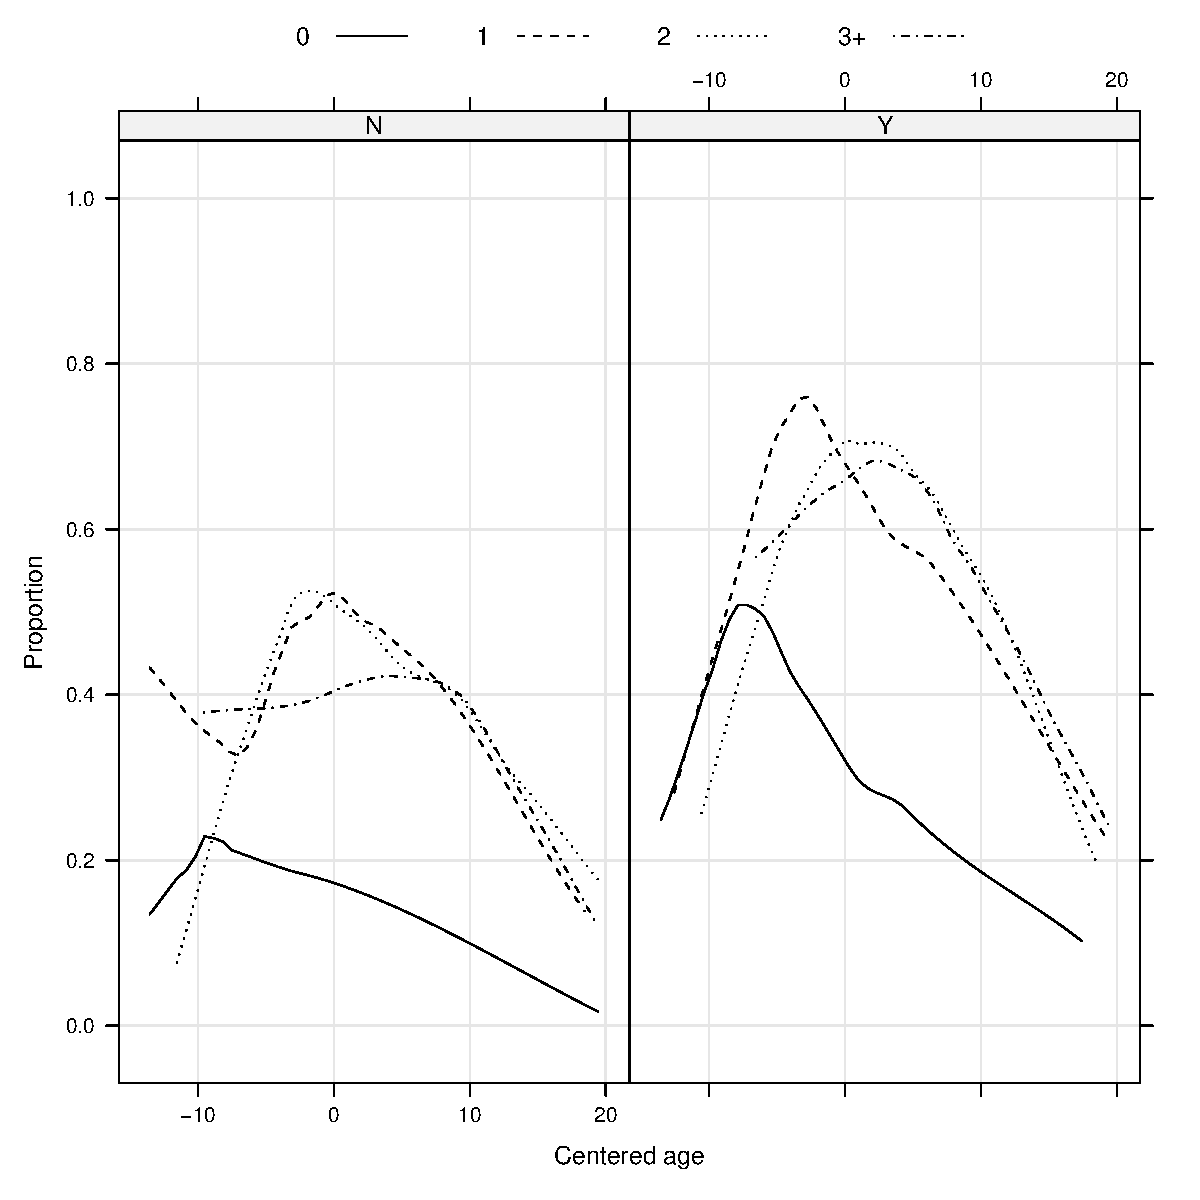
\includegraphics[width=\textwidth]{figs/SoftRev-Contra1}
  \caption{Scatterplot smoother curves of the use of artificial
    contraception versus age for women in the Bangladesh fertility
    survey. The panel on the left depicts the proportion for rural
    women and the panel on the right depicts the proportion for urban
    women.}
  \label{fig:Contra1}
\end{figure}
shows that this is not the case.  Indeed the proportion of women using
artificial contraception is more like a quadratic in age.  Very young
women and older women are less likely to use artificial contraception.

We also see that the differences according to the number of live
children are predominantly differences between those women who have
live children and those who don't.


\subsection{Reformulated models}
\label{sec:ContraReformulated}

We include a quadratic term in \code{age}
\begin{Schunk}
\begin{Sinput}
> (Cm6 <- lmer(use ~ age + I(age^2) + urban + livch + (1 | district), 
+     Contraception, binomial, method = "AGQ"))
\end{Sinput}
\begin{Soutput}
Generalized linear mixed model fit using AGQ 
Formula: use ~ age + I(age^2) + urban + livch + (1 | district) 
   Data: Contraception 
 Family: binomial(logit link)
      AIC      BIC    logLik deviance
 2390.486 2440.592 -1186.243 2372.486
Random effects:
     Groups        Name    Variance    Std.Dev. 
   district (Intercept)     0.22965     0.47922 
# of obs: 1934, groups: district, 60

Estimated scale (compare to 1)  1.027380 

Fixed effects:
               Estimate  Std. Error z value  Pr(>|z|)
(Intercept) -1.01594748  0.17423926 -5.8308 5.518e-09
age          0.00350981  0.00921331  0.3809    0.7032
I(age^2)    -0.00458880  0.00072305 -6.3465 2.203e-10
urbanY       0.68389839  0.11977356  5.7099 1.130e-08
livch1       0.80217960  0.16191417  4.9544 7.257e-07
livch2       0.90132794  0.18483015  4.8765 1.080e-06
livch3+      0.90006573  0.18546304  4.8531 1.216e-06
\end{Soutput}
\begin{Sinput}
> anova(Cm1, Cm6)
\end{Sinput}
\begin{Soutput}
Data: Contraception
Models:
Cm1: use ~ age + urban + livch + (1 | district)
Cm6: use ~ age + I(age^2) + urban + livch + (1 | district)
    Df     AIC     BIC  logLik  Chisq Chi Df Pr(>Chisq)
Cm1  8  2429.7  2474.2 -1206.8                         
Cm6  9  2390.5  2440.6 -1186.2 41.178      1  1.390e-10
\end{Soutput}
\end{Schunk}
and we see that, as indicated by the plots, the quadratic term is highly significant.

We can check if the differences in the number of live children is
primarily the difference between no children and any children by
fitting a model with the indicator \code{livch == 0} as one of the
terms in the fixed effects.
\begin{Schunk}
\begin{Sinput}
> (Cm7 <- lmer(use ~ age + I(age^2) + urban + (livch == 0) + (1 | 
+     district), Contraception, binomial, method = "AGQ"))
\end{Sinput}
\begin{Soutput}
Generalized linear mixed model fit using AGQ 
Formula: use ~ age + I(age^2) + urban + (livch == 0) + (1 | district) 
   Data: Contraception 
 Family: binomial(logit link)
      AIC      BIC    logLik deviance
 2386.943 2425.914 -1186.471 2372.943
Random effects:
     Groups        Name    Variance    Std.Dev. 
   district (Intercept)     0.22830     0.47781 
# of obs: 1934, groups: district, 60

Estimated scale (compare to 1)  1.027534 

Fixed effects:
                  Estimate  Std. Error z value  Pr(>|z|)
(Intercept)    -0.14136696  0.10169380 -1.3901    0.1645
age             0.00617737  0.00782799  0.7891    0.4300
I(age^2)       -0.00466050  0.00071423 -6.5252 6.792e-11
urbanY          0.67973583  0.11956250  5.6852 1.307e-08
livch == 0TRUE -0.84656062  0.14706981 -5.7562 8.604e-09
\end{Soutput}
\begin{Sinput}
> anova(Cm6, Cm7)
\end{Sinput}
\begin{Soutput}
Data: Contraception
Models:
Cm7: use ~ age + I(age^2) + urban + (livch == 0) + (1 | district)
Cm6: use ~ age + I(age^2) + urban + livch + (1 | district)
    Df     AIC     BIC  logLik  Chisq Chi Df Pr(>Chisq)
Cm7  7  2386.9  2425.9 -1186.5                         
Cm6  9  2390.5  2440.6 -1186.2 0.4572      2     0.7956
\end{Soutput}
\end{Schunk}

Based on the change in the log-likelihood the simpler model is
adequate.  We add a variable \code{children} which is an indicator of
any children versus no children to the data set
\begin{Schunk}
\begin{Sinput}
> Contraception$children <- with(Contraception, factor(ifelse(livch == 
+     0, "N", "Y")))
\end{Sinput}
\end{Schunk}
so we can check for an interaction with the \code{urban} factor.
\begin{Schunk}
\begin{Sinput}
> (Cm8 <- lmer(use ~ age + I(age^2) + urban * children + (1 | district), 
+     Contraception, binomial, method = "AGQ"))
\end{Sinput}
\begin{Soutput}
Generalized linear mixed model fit using AGQ 
Formula: use ~ age + I(age^2) + urban * children + (1 | district) 
   Data: Contraception 
 Family: binomial(logit link)
      AIC      BIC    logLik deviance
 2387.868 2432.406 -1185.934 2371.868
Random effects:
     Groups        Name    Variance    Std.Dev. 
   district (Intercept)      0.2274     0.47686 
# of obs: 1934, groups: district, 60

Estimated scale (compare to 1)  1.027846 

Fixed effects:
                    Estimate  Std. Error z value  Pr(>|z|)
(Intercept)      -1.07644093  0.19034365 -5.6552 1.556e-08
age               0.00554896  0.00785464  0.7065    0.4799
I(age^2)         -0.00460180  0.00071638 -6.4237 1.330e-10
urbanY            0.87145946  0.22228750  3.9204 8.840e-05
childrenY         0.95142628  0.18072909  5.2644 1.407e-07
urbanY:childrenY -0.25574959  0.25002441 -1.0229    0.3064
\end{Soutput}
\end{Schunk}
The interaction is not significant.

We can check if there is significant variation by district in the
effect of urban versus rural or in the effect of any children versus
no children by fitting further models
\begin{Schunk}
\begin{Sinput}
> (Cm9 <- lmer(use ~ age + I(age^2) + urban + children + (urban | 
+     district), Contraception, binomial, method = "Laplace"))
\end{Sinput}
\begin{Soutput}
Generalized linear mixed model fit using Laplace 
Formula: use ~ age + I(age^2) + urban + children + (urban | district) 
   Data: Contraception 
 Family: binomial(logit link)
      AIC      BIC    logLik deviance
 2378.938 2429.044 -1180.469 2360.938
Random effects:
 Groups   Name        Variance Std.Dev. Corr   
 district (Intercept) 0.38334  0.61914         
          urbanY      0.54648  0.73924  -0.794 
# of obs: 1934, groups: district, 60

Estimated scale (compare to 1)  1.015014 

Fixed effects:
              Estimate Std. Error z value  Pr(>|z|)
(Intercept) -1.0338419  0.1783648 -5.7962 6.783e-09
age          0.0057762  0.0079049  0.7307     0.465
I(age^2)    -0.0045492  0.0007210 -6.3096 2.797e-10
urbanY       0.7676803  0.1626603  4.7195 2.364e-06
childrenY    0.8712301  0.1484547  5.8687 4.393e-09
\end{Soutput}
\begin{Sinput}
> anova(Cm7, Cm9)
\end{Sinput}
\begin{Soutput}
Data: Contraception
Models:
Cm7: use ~ age + I(age^2) + urban + (livch == 0) + (1 | district)
Cm9: use ~ age + I(age^2) + urban + children + (urban | district)
    Df     AIC     BIC  logLik  Chisq Chi Df Pr(>Chisq)
Cm7  7  2386.9  2425.9 -1186.5                         
Cm9  9  2378.9  2429.0 -1180.5 12.005      2   0.002472
\end{Soutput}
\begin{Sinput}
> (Cm10 <- lmer(use ~ age + I(age^2) + urban + children + (children | 
+     district), Contraception, binomial, method = "Laplace"))
\end{Sinput}
\begin{Soutput}
Generalized linear mixed model fit using Laplace 
Formula: use ~ age + I(age^2) + urban + children + (children | district) 
   Data: Contraception 
 Family: binomial(logit link)
      AIC      BIC    logLik deviance
 2387.888 2437.994 -1184.944 2369.888
Random effects:
 Groups   Name        Variance Std.Dev. Corr   
 district (Intercept) 0.46455  0.68158         
          childrenY   0.29709  0.54506  -0.727 
# of obs: 1934, groups: district, 60

Estimated scale (compare to 1)  1.013278 

Fixed effects:
               Estimate  Std. Error z value  Pr(>|z|)
(Intercept) -1.06057305  0.18544077 -5.7192 1.070e-08
age          0.00696144  0.00789076  0.8822    0.3777
I(age^2)    -0.00464493  0.00071791 -6.4700 9.798e-11
urbanY       0.69950039  0.12042808  5.8084 6.305e-09
childrenY    0.91440356  0.17237364  5.3048 1.128e-07
\end{Soutput}
\begin{Sinput}
> anova(Cm7, Cm10)
\end{Sinput}
\begin{Soutput}
Data: Contraception
Models:
Cm7: use ~ age + I(age^2) + urban + (livch == 0) + (1 | district)
Cm10: use ~ age + I(age^2) + urban + children + (children | district)
     Df     AIC     BIC  logLik  Chisq Chi Df Pr(>Chisq)
Cm7   7  2386.9  2425.9 -1186.5                         
Cm10  9  2387.9  2438.0 -1184.9 3.0549      2     0.2171
\end{Soutput}
\end{Schunk}

Variation due to district in the effect of any children versus no
children does not appear to be significant but there is a significant
variation in the effect of urban versus rural.  It is interesting that
AIC (Akaike's Information Criterion) and BIC (Schwartz's Bayesian
Information Criterion) lead to different conclusions in the comparison
of \code{Cm7} versus \code{Cm9}.  For both these criteria the
preferred model is the one with the lower value of the criterion.
Hence, AIC prefers \code{Cm9} and BIC prefers \code{Cm7}.  The BIC
criterion puts a heavier penalty on having a greater number of parameters.

At present the code for creating a Markov Chain Monte Carlo sample
from the distribution of the parameters in a generalized linear mixed
model does not allow for random effects of dimension greater than one
so we produce a sample from the posterior distribution of the
parameters in model \code{Cm11}
\begin{Schunk}
\begin{Sinput}
> (Cm11 <- lmer(use ~ age + I(age^2) + urban + children + (1 | 
+     district), Contraception, binomial, method = "AGQ"))
\end{Sinput}
\begin{Soutput}
Generalized linear mixed model fit using AGQ 
Formula: use ~ age + I(age^2) + urban + children + (1 | district) 
   Data: Contraception 
 Family: binomial(logit link)
      AIC      BIC    logLik deviance
 2386.918 2425.889 -1186.459 2372.918
Random effects:
     Groups        Name    Variance    Std.Dev. 
   district (Intercept)     0.22822     0.47773 
# of obs: 1934, groups: district, 60

Estimated scale (compare to 1)  1.027538 

Fixed effects:
               Estimate  Std. Error z value  Pr(>|z|)
(Intercept) -1.00289039  0.16778919 -5.9771 2.272e-09
age          0.00643755  0.00782799  0.8224    0.4109
I(age^2)    -0.00466413  0.00071423 -6.5303 6.565e-11
urbanY       0.69212653  0.11956250  5.7888 7.088e-09
childrenY    0.85816677  0.14706981  5.8351 5.376e-09
\end{Soutput}
\begin{Sinput}
> Cs11 <- mcmcsamp(Cm11, 10000, trans = FALSE)
\end{Sinput}
\end{Schunk}
Density plots (Figure~\ref{fig:Contra2})
\begin{figure}[tbp]
  \centering
  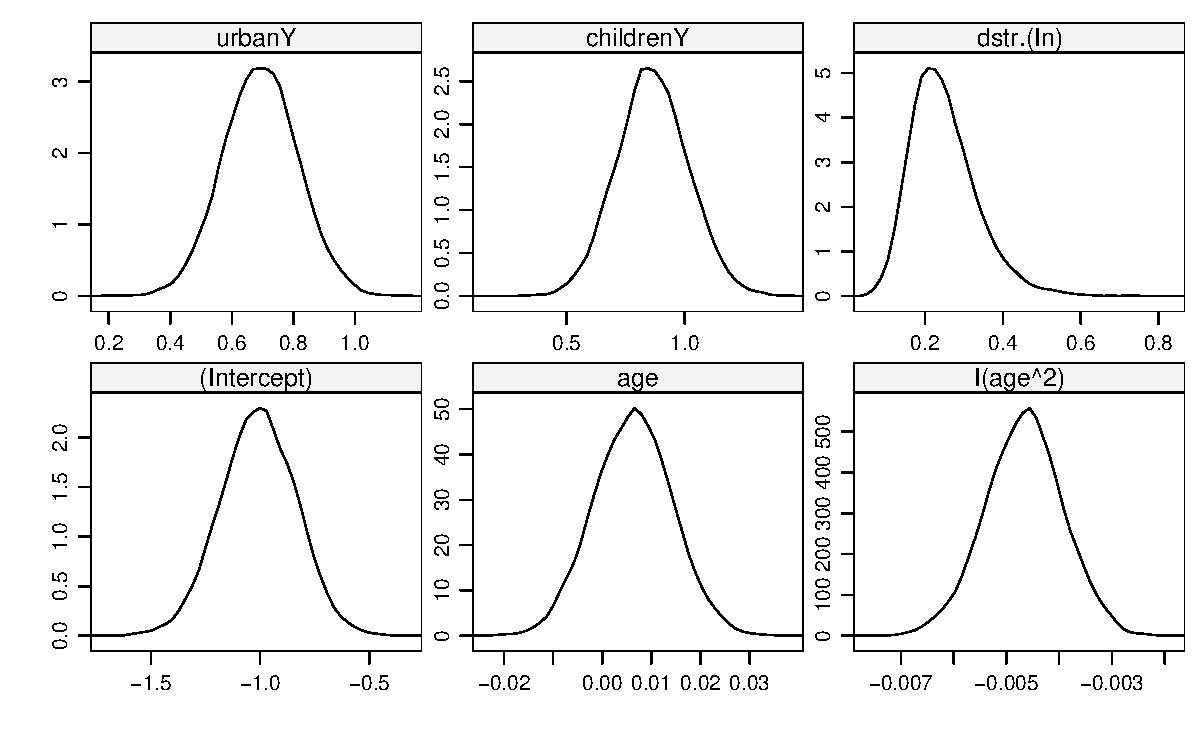
\includegraphics[width=\textwidth]{figs/SoftRev-Contra2}
  \caption{Plots of the estimated posterior probability densities from
    a Markov Chain Monte Carlo sample of the parameters in the model
    \code{Cm11} fit to the \code{Contraception} data.} 
  \label{fig:Contra2}
\end{figure}
and normal probability plots (Figure~\ref{fig:Contra3})
\begin{figure}[tbp]
  \centering
  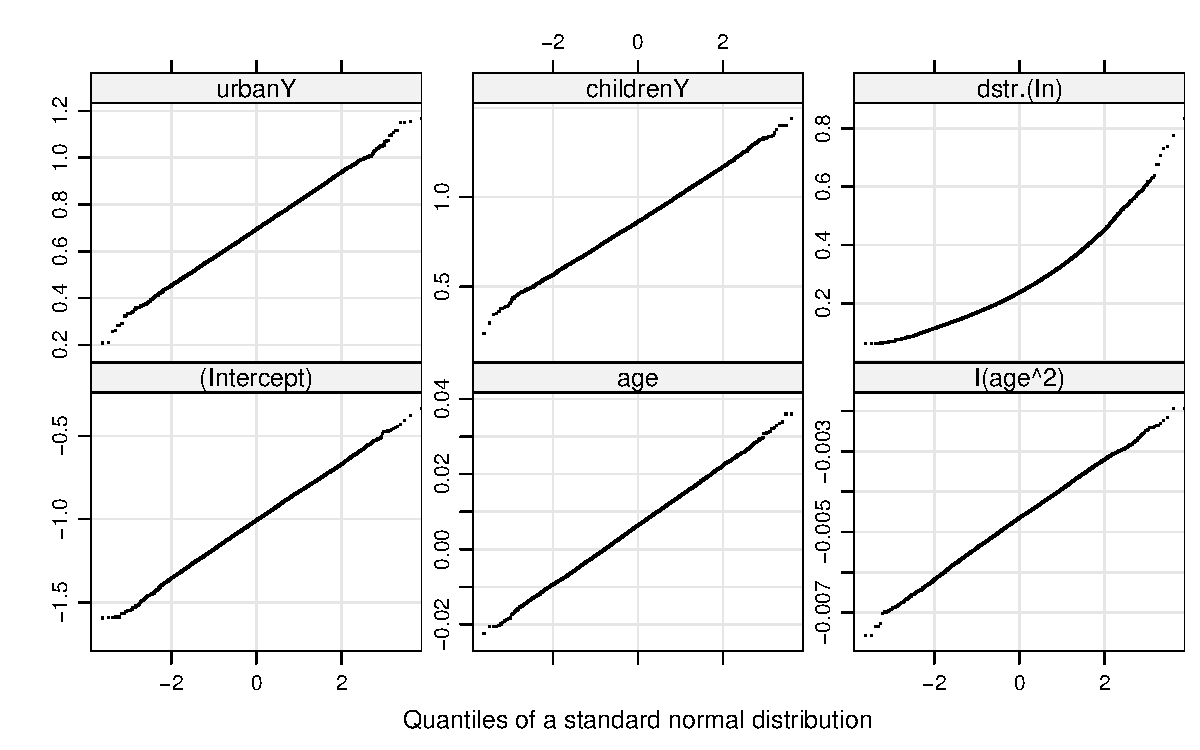
\includegraphics[width=\textwidth]{figs/SoftRev-Contra3}
  \caption{Normal probability plots of the Markov Chain Monte Carlo
    samples from the posterior densities of the parameters in the
    model \code{Cm11} fit to the \code{Contraception} data.} 
  \label{fig:Contra3}
\end{figure}

for this sample show that the fixed-effects
parameters are very well approximated by a normal distribution but the
variance of the random effects shows noticeable skewness.

\section{Growth curve model for repeated measures data}
\label{sec:GrowthCurve}

\begin{Schunk}
\begin{Sinput}
> str(Oxboys)
\end{Sinput}
\begin{Soutput}
`data.frame':	234 obs. of  4 variables:
 $ Subject : Factor w/ 26 levels "1","10","11",..: 1 1 1 1 1 1 1 1 1 12 ...
 $ age     : num  -1.0000 -0.7479 -0.4630 -0.1643 -0.0027 ...
 $ height  : num  140 143 145 147 148 ...
 $ Occasion: Factor w/ 9 levels "1","2","3","4",..: 1 2 3 4 5 6 7 8 9 1 ...
 - attr(*, "ginfo")=List of 7
  ..$ formula     :Class 'formula' length 3 height ~ age | Subject
  .. .. ..- attr(*, ".Environment")=length 30 <environment> 
  ..$ order.groups: logi TRUE
  ..$ FUN         :function (x)  
  .. ..- attr(*, "source")= chr "function (x) max(x, na.rm = TRUE)"
  ..$ outer       : NULL
  ..$ inner       : NULL
  ..$ labels      :List of 2
  .. ..$ age   : chr "Centered age"
  .. ..$ height: chr "Height"
  ..$ units       :List of 1
  .. ..$ height: chr "(cm)"
\end{Soutput}
\begin{Sinput}
> system.time(mX1 <- lmer(height ~ age + I(age^2) + I(age^3) + 
+     I(age^4) + (age + I(age^2) | Subject), Oxboys), gc = TRUE)
\end{Sinput}
\begin{Soutput}
[1] 0.07 0.00 0.06 0.00 0.00
\end{Soutput}
\begin{Sinput}
> summary(mX1)
\end{Sinput}
\begin{Soutput}
Linear mixed-effects model fit by REML
Formula: height ~ age + I(age^2) + I(age^3) + I(age^4) + (age + I(age^2) |      Subject) 
   Data: Oxboys 
      AIC     BIC    logLik MLdeviance REMLdeviance
 651.9081 693.372 -313.9541   625.3593     627.9081
Random effects:
 Groups   Name        Variance Std.Dev. Corr        
 Subject  (Intercept) 64.03492 8.00218              
          age          2.86417 1.69239  0.614       
          I(age^2)     0.67429 0.82115  0.215 0.658 
 Residual              0.21737 0.46623              
# of obs: 234, groups: Subject, 26

Fixed effects:
             Estimate Std. Error  DF t value  Pr(>|t|)
(Intercept) 149.01887    1.57037 229 94.8944 < 2.2e-16
age           6.17418    0.35650 229 17.3187 < 2.2e-16
I(age^2)      1.12823    0.35144 229  3.2103  0.001516
I(age^3)      0.45385    0.16246 229  2.7937  0.005653
I(age^4)     -0.37690    0.30018 229 -1.2556  0.210552

Correlation of Fixed Effects:
         (Intr) age    I(g^2) I(g^3)
age       0.572                     
I(age^2)  0.076  0.264              
I(age^3) -0.001 -0.340  0.025       
I(age^4)  0.021  0.016 -0.857 -0.021
\end{Soutput}
\begin{Sinput}
> system.time(mX2 <- lmer(height ~ poly(age, 4) + (age + I(age^2) | 
+     Subject), Oxboys), gc = TRUE)
\end{Sinput}
\begin{Soutput}
[1] 0.11 0.00 0.10 0.00 0.00
\end{Soutput}
\begin{Sinput}
> summary(mX2)
\end{Sinput}
\begin{Soutput}
Linear mixed-effects model fit by REML
Formula: height ~ poly(age, 4) + (age + I(age^2) | Subject) 
   Data: Oxboys 
      AIC      BIC    logLik MLdeviance REMLdeviance
 640.8686 682.3324 -308.4343   625.3593     616.8686
Random effects:
 Groups   Name        Variance Std.Dev. Corr        
 Subject  (Intercept) 64.03492 8.00218              
          age          2.86417 1.69239  0.614       
          I(age^2)     0.67429 0.82115  0.215 0.658 
 Residual              0.21737 0.46623              
# of obs: 234, groups: Subject, 26

Fixed effects:
               Estimate Std. Error  DF t value  Pr(>|t|)
(Intercept)   149.51976    1.59031 229 94.0193 < 2.2e-16
poly(age, 4)1  64.54095    3.32786 229 19.3941 < 2.2e-16
poly(age, 4)2   4.20322    1.02361 229  4.1063 5.597e-05
poly(age, 4)3   1.29077    0.46628 229  2.7682  0.006098
poly(age, 4)4  -0.58547    0.46630 229 -1.2556  0.210552

Correlation of Fixed Effects:
            (Intr) p(,4)1 p(,4)2 p(,4)3
poly(ag,4)1 0.631                      
poly(ag,4)2 0.230  0.583               
poly(ag,4)3 0.000  0.000  0.000        
poly(ag,4)4 0.000  0.000  0.000  0.000 
\end{Soutput}
\end{Schunk}

\section{Cross-classification model}
\label{sec:CrossClassified}

\begin{Schunk}
\begin{Sinput}
> str(ScotsSec)
\end{Sinput}
\begin{Soutput}
`data.frame':	3435 obs. of  6 variables:
 $ verbal : num  11 0 -14 -6 -30 -17 -17 -11 -9 -19 ...
 $ attain : num  10 3 2 3 2 2 4 6 4 2 ...
 $ primary: Factor w/ 148 levels "1","2","3","4",..: 1 1 1 1 1 1 1 1 1 1 ...
 $ sex    : Factor w/ 2 levels "M","F": 1 2 1 1 2 2 2 1 1 1 ...
 $ social : num  0 0 0 20 0 0 0 0 0 0 ...
 $ second : Factor w/ 19 levels "1","2","3","4",..: 9 9 9 9 9 9 1 1 9 9 ...
\end{Soutput}
\begin{Sinput}
> system.time(mS1 <- lmer(attain ~ sex + (1 | primary) + (1 | second), 
+     ScotsSec), gc = TRUE)
\end{Sinput}
\begin{Soutput}
[1] 0.11 0.00 0.12 0.00 0.00
\end{Soutput}
\begin{Sinput}
> summary(mS1)
\end{Sinput}
\begin{Soutput}
Linear mixed-effects model fit by REML
Formula: attain ~ sex + (1 | primary) + (1 | second) 
   Data: ScotsSec 
      AIC      BIC    logLik MLdeviance REMLdeviance
 17137.91 17168.62 -8563.956   17123.49     17127.91
Random effects:
 Groups   Name        Variance Std.Dev.
 primary  (Intercept) 1.10962  1.0534  
 second   (Intercept) 0.36966  0.6080  
 Residual             8.05511  2.8382  
# of obs: 3435, groups: primary, 148; second, 19

Fixed effects:
              Estimate Std. Error   DF t value  Pr(>|t|)
(Intercept) 5.2552e+00 1.8432e-01 3433 28.5108 < 2.2e-16
sexF        4.9851e-01 9.8255e-02 3433  5.0737 4.109e-07

Correlation of Fixed Effects:
     (Intr)
sexF -0.264
\end{Soutput}
\end{Schunk}

\bibliography{MlmSoftRev}
\end{document}
